\documentclass[12pt,a4paper]{article}
\usepackage[utf8]{inputenc}
\usepackage[T1]{fontenc}
\usepackage{amsmath}
\usepackage{amsfonts}
\usepackage{amssymb}
\usepackage{graphicx}
\usepackage{longtable}
\usepackage[left=2.5cm,right=2.5cm,top=2.5cm,bottom=2.5cm]{geometry}
\usepackage[round,authoryear]{natbib}  % Specify author-year citation style
\usepackage{hyperref}
\usepackage{xr}                % For cross-referencing between documents
\usepackage{cleveref}          % For intelligent cross-referencing
\usepackage{pdflscape}         % For landscape pages
\usepackage{mdframed}          % For creating boxed environments
\usepackage{xcolor}            % For custom colors
\usepackage{tikz}             % For creating diagrams and flowcharts
\usetikzlibrary{positioning}  % For relative positioning in TikZ
\usetikzlibrary{shapes.geometric}  % For geometric shapes in TikZ
\usepackage{lineno}

% Define custom prompt environment
\definecolor{promptbg}{RGB}{250,250,250}
\definecolor{promptframe}{RGB}{200,200,200}
\newmdenv[
    linewidth=1pt,
    backgroundcolor=promptbg,
    linecolor=promptframe,
    leftmargin=1em,
    rightmargin=1em,
    innerleftmargin=1em,
    innerrightmargin=1em,
    innertopmargin=1em,
    innerbottommargin=1em,
    skipabove=1em,
    skipbelow=1em
]{prompt}

% Configure hyperref after other packages
\hypersetup{
    colorlinks=true,
    linkcolor=blue,
    filecolor=magenta,
    urlcolor=cyan,
    citecolor=blue
}

\title{Automated Diet Matrix Construction for Marine Ecosystem Models Using Generative AI}

\author{Scott Spillias\textsuperscript{1,2}\thanks{Corresponding author: scott.spillias@csiro.au} \and
Beth Fulton\textsuperscript{1,2} \and
Fabio Boschetti\textsuperscript{2,3} \and
Joanna Strzelecki\textsuperscript{3} \and
Rowan Trebilco\textsuperscript{1,2}}

\date{\today}  % Use current date or remove for no date

% Author affiliations
\newcommand{\affiliations}{
\noindent\textsuperscript{1}CSIRO Environment, Hobart, Australia\\
\textsuperscript{2}Centre for Marine Socio-Ecology, University of Tasmania, Hobart, Australia\\
\textsuperscript{3}CSIRO Environment, IOMRC Crawley, Australia\\
\textsuperscript{4}CSIRO Environment, St. Lucia, Australia
}

\begin{document}
\linenumbers
\maketitle
\affiliations

\begin{abstract}
This study introduces and validates a novel AI-driven framework for automated species grouping and diet matrix generation in Ecopath with Ecosim (EwE) ecosystem models, addressing a critical bottleneck in model development. We evaluate the framework across three contrasting Australian marine regions (Shelf and Offshore regions of South-East Tasmania and the Northern Territory), processing over 41,000 species through multiple validation iterations. The framework successfully condensed 63 potential functional groups into 34-36 region-specific groups, achieving high classification stability (>99\% consistency) for most species. Notably, the framework demonstrated robust performance in the South East offshore region with only 0.03\% inconsistent classifications, while showing greater variability in complex tropical systems (1\% inconsistent classifications). Higher trophic level species maintained consistent classifications across all runs, with the framework identifying 235-327 significant predator-prey interactions per region at >70\% consistency. This systematic validation reveals that while the framework can reliably automate species grouping, its performance varies predictably with ecosystem complexity and data availability. These findings provide quantitative evidence for the framework's ability to create repeatable components for ecosystem model development. Our results demonstrate the potential for AI to significantly reduce model development time, offering a practical pathway to expand the application of ecosystem-based management across diverse marine environments. We offer a pathway towards further validation of this framework to ensure ecological accuracy.
\end{abstract}

Ecosystem-based fisheries management (EBFM) has emerged as a critical policy goal for ocean management agencies worldwide \citep{FAO2003, EuropeanCommission2013, NOAA2016}. The practical implementation of ecosystem approaches to management requires ecosystem modeling within the context of natural resource management processes \citep{Collie2016}. Among these approaches, mass-balance models that track biomass flows between producers, consumers, predators, and fisheries have become foundational tools for understanding ecosystem structure and function \citep{Christensen2004}.

Ecopath with Ecosim (EwE) represents one of the most widely used food web modeling approaches in marine ecosystems \citep{Christensen2004, Colleter2015}. The model explicitly incorporates trophic interactions among multiple species and functional groups while maintaining mass conservation constraints across the broader food web. This makes EwE particularly valuable for quantifying trade-offs arising from natural or anthropogenic perturbations and assessing cumulative impacts of multiple stressors on marine ecosystems \citep{Coll2015, Villasante2016}.

A critical aspect of ecosystem modeling is the validation of model components and outputs. As model complexity increases to reflect biological realism, there is an unavoidable concurrent increase in scientific uncertainty due to limited knowledge of functional relationships \citep{PlaganyiButterworth2004}. This is particularly relevant for species grouping decisions, which form the foundation of any ecosystem model's structure. The reliability of ecosystem models depends heavily on appropriate species grouping that accurately represents the ecological roles and trophic interactions within the system.

Recent advances in artificial intelligence and machine learning present new opportunities for automating and validating species grouping decisions in ecosystem models. However, these approaches require rigorous validation to ensure they capture meaningful ecological relationships. This validation is essential as grouping decisions can significantly impact model behavior and subsequent management recommendations \citep{Heymans2016, Link2010}.

The validation of AI-based species grouping must consider both the ecological principles of functional group formation and the geographic context in which these groups operate. Marine ecosystems exhibit significant spatial heterogeneity in their physical, chemical, and biological characteristics, which directly influences species distributions, interactions, and functional roles \citep{Longhurst2007}. A species that serves as a key predator in one region may play a different ecological role in another due to variations in habitat availability, prey distributions, or environmental conditions. Therefore, validating AI-generated functional groups across distinct geographic regions is crucial for several reasons:

1. It tests the AI's ability to recognize and account for regional differences in ecosystem structure and function
2. It ensures that species groupings reflect local ecological contexts rather than applying a one-size-fits-all approach
3. It validates the AI's capacity to incorporate region-specific environmental and oceanographic factors that influence species' ecological roles
4. It helps identify potential biases or limitations in the AI's understanding of how geographic variation affects trophic relationships and ecosystem dynamics

This analysis examines the reliability and consistency of automated species grouping across three distinct marine regions: the Northern Territory, South East Inshore, and South East Offshore. Our validation framework addresses three key aims:

1. To assess AI models' understanding of regional marine ecosystems through their ability to generate accurate and comprehensive ecosystem descriptions
2. To evaluate the consistency of functional group generation across different AI models and marine regions
3. To analyze the ecological validity of AI-generated functional groups by comparing them against established ecological principles and known regional characteristics

By leveraging multiple AI models and comparing their performance across different ecological contexts, we aim to assess the robustness of automated grouping approaches and their potential role in ecosystem-based management.

\section{Methodology}

We evaluated seven AI models (Claude (Anthropic), AWS Claude, Google Gemini, Gemma2, Gemma7, Llama3, and Mixtral) across three distinct marine regions: the Northern Territory (tropical waters), South East Inshore (temperate coastal waters), and South East Offshore (temperate oceanic waters). We defined each region using shapefiles containing precise geographical boundaries, which we converted to GeoJSON format for processing (Figure \ref{fig:validation_regions}).

\begin{figure}[H]
    \centering
    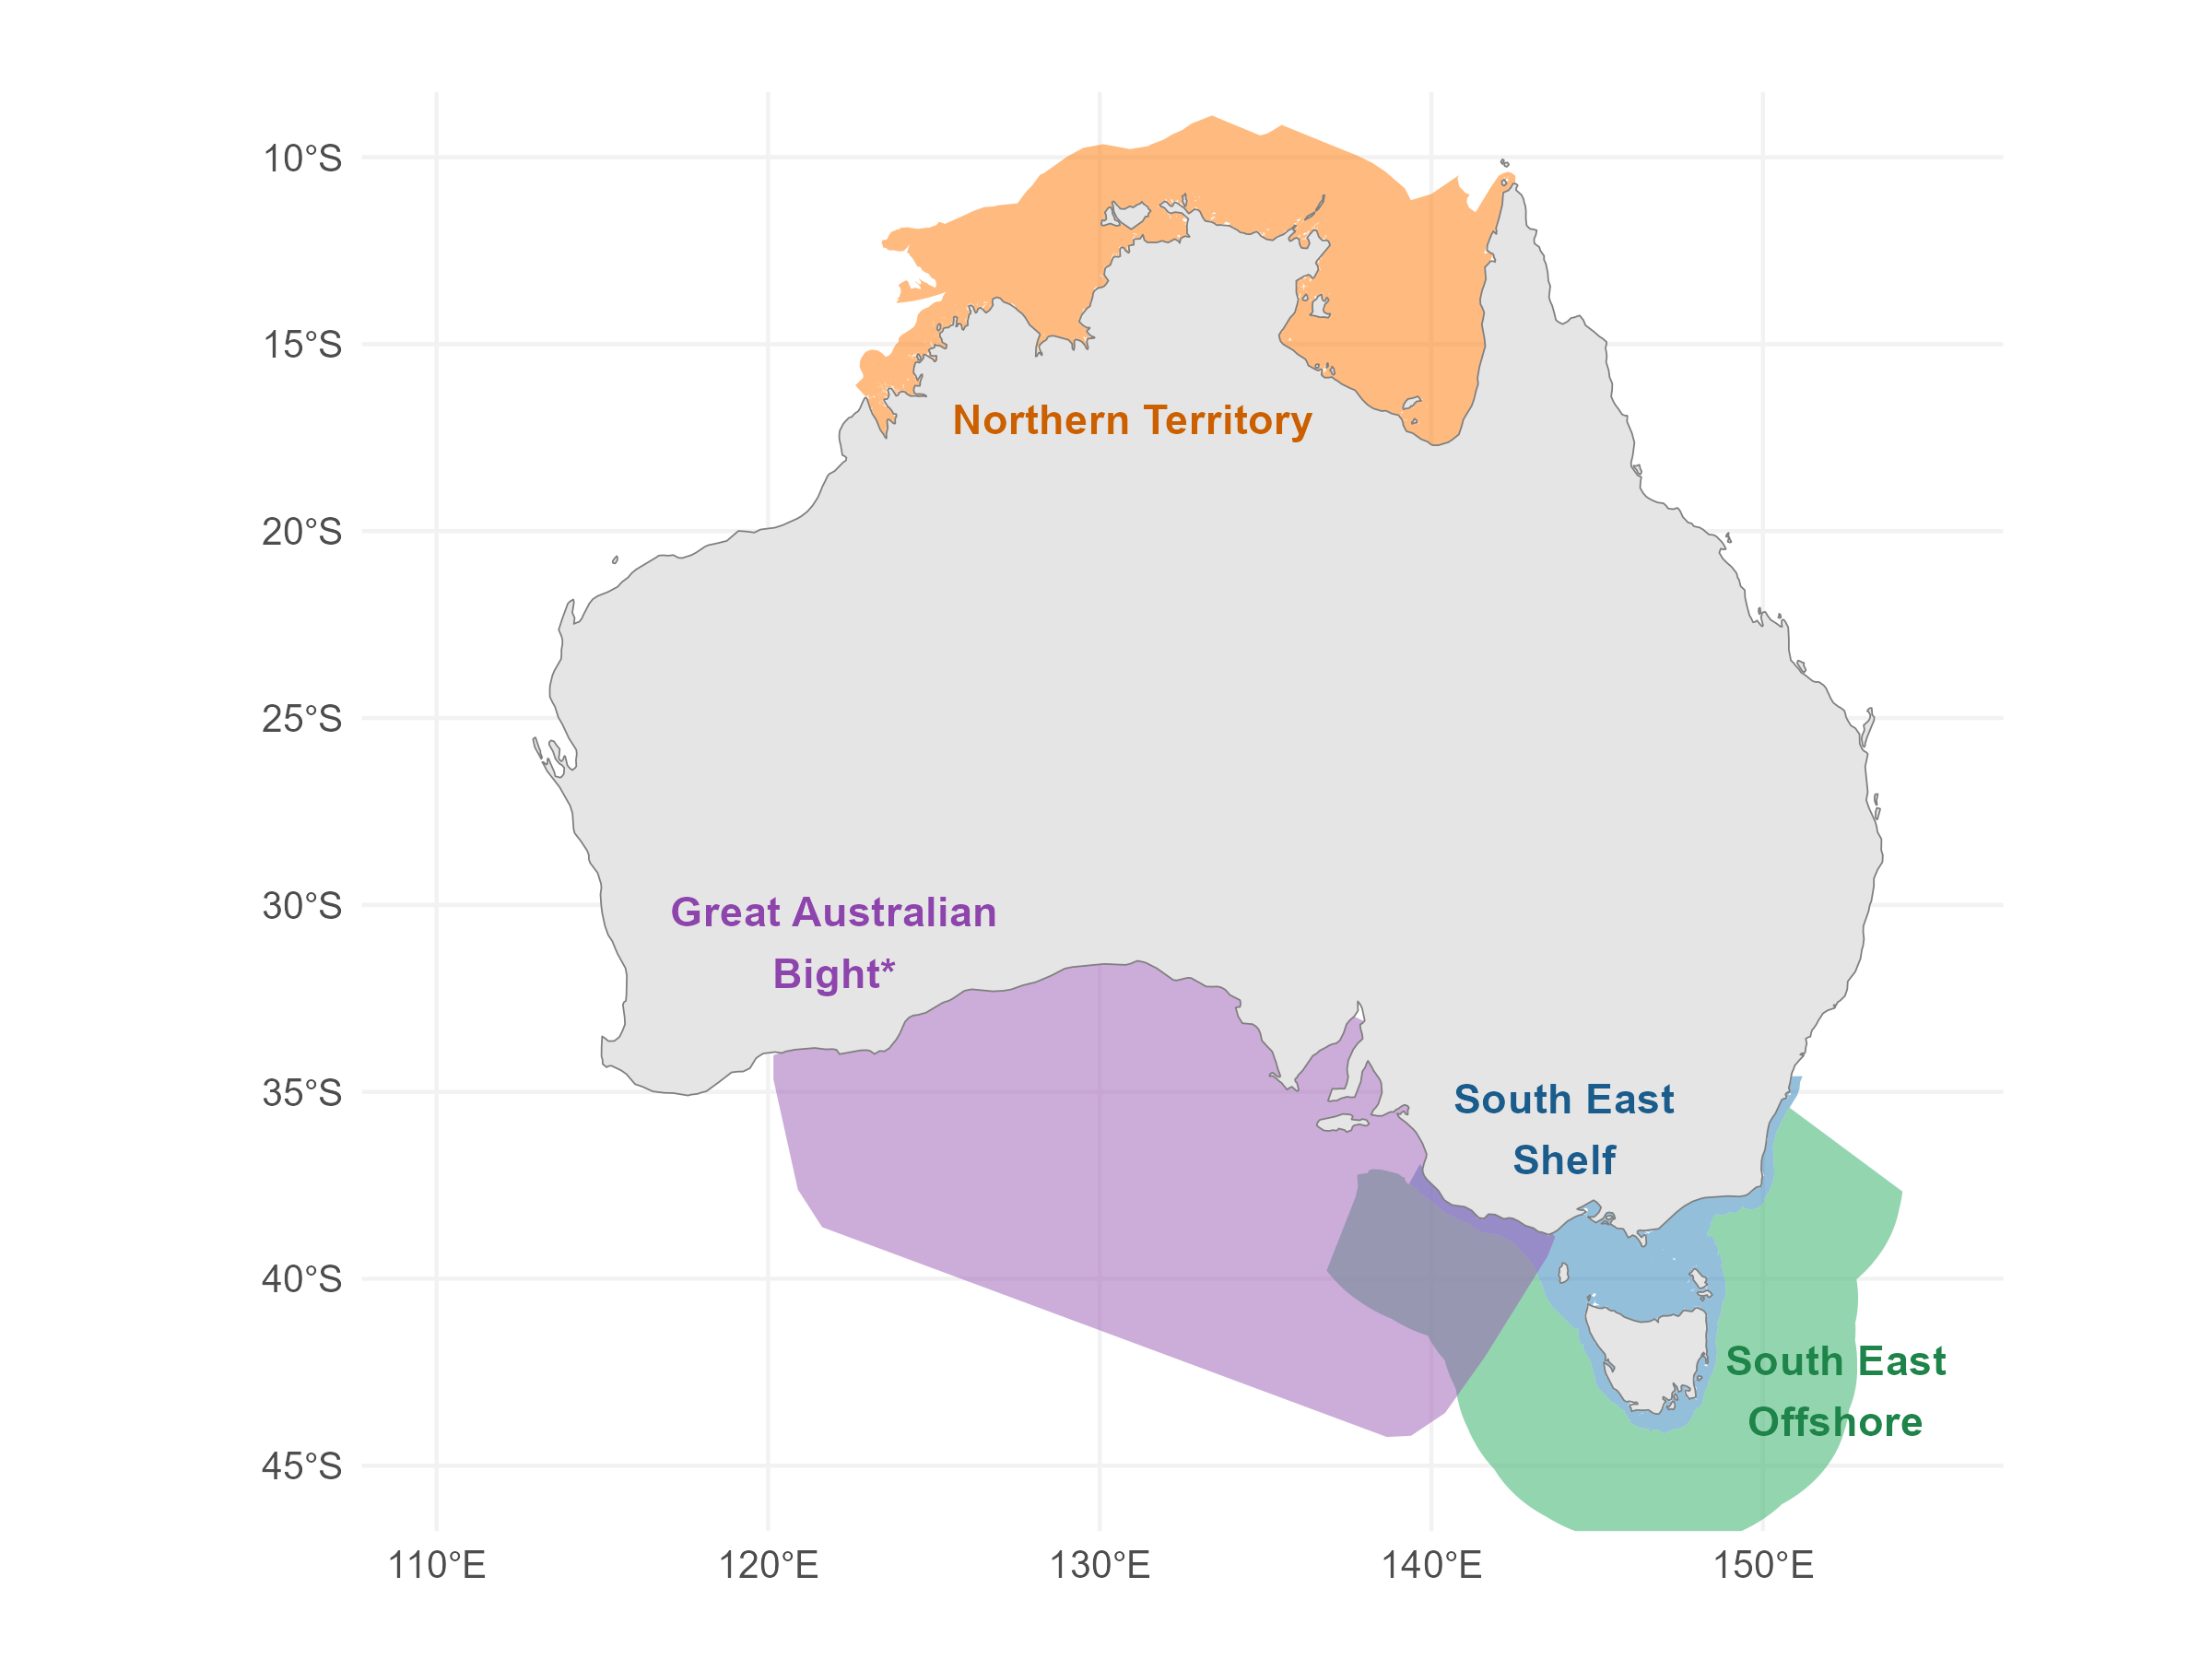
\includegraphics[width=\textwidth]{validation_regions.png}
    \caption{Validation regions used in the study: Northern Territory (tropical), South East Inshore (temperate coastal), and South East Offshore (temperate oceanic).}
    \label{fig:validation_regions}
\end{figure}

\subsection{Regional Ecosystem Understanding}
To assess AI models' comprehension of regional marine ecosystems, we employed a standardized prompting protocol (see Supplementary Material, AI Prompting Protocol). For each region, we first extracted geographic extents from the GeoJSON files to define the study area boundaries. We then prompted each model to provide detailed ecosystem descriptions encompassing geographic location, notable features, marine environment type, oceanographic conditions, habitat types, and key ecological characteristics.

We evaluated these AI-generated descriptions through multiple criteria:
\begin{itemize}
    \item Comprehensiveness of physical and biological characteristics
    \item Accuracy compared to known oceanographic patterns
    \item Alignment with regional ecological surveys
    \item Consistency with documented biodiversity patterns
    \item Accuracy of described seasonal dynamics
\end{itemize}

\subsection{Functional Group Generation Consistency}
We implemented an iterative validation protocol to assess the consistency of functional group generation. The process involved a two-stage approach for each region and AI model combination. First, we provided the AI model with the validated ecosystem description and a comprehensive template of possible functional groups (see Supplementary Material, Grouping Template). This template served as a reference point but did not constrain the models, which could create new groups or modify existing ones based on regional characteristics.

The group generation process followed specific ecological criteria:
\begin{itemize}
    \item Groups could represent individual species or collections of species sharing similar ecological functions
    \item Species were grouped based on similar growth rates, consumption rates, diets, habitats, and predators
    \item Groupings prioritized ecological niche similarity over taxonomic relationships
    \item Higher resolution groupings were maintained for species related to the research focus
    \item Broader functional groups were used for species with less direct relevance to the study objectives
\end{itemize}

For each region-model combination, we conducted five independent iterations. Each iteration generated a complete set of functional groups, with results stored in a standardized JSON format including detailed descriptions of each group's ecological role. We tracked group occurrence across iterations and created group occurrence matrices. To quantify consistency, we calculated a consistency score for each functional group using:

\[
\text{Consistency Score} = \frac{\text{Number of occurrences of group}}{\text{Total number of iterations}}
\]

We generated heatmaps to visualize consistency patterns across models and regions.

\subsection{Ecological Validity Assessment}
We evaluated the ecological validity of AI-generated functional groups by analyzing their adherence to established ecological principles. For each generated group set, we assessed:
\begin{itemize}
    \item Coverage across all major trophic levels
    \item Representation of key ecological roles
    \item Appropriateness of species groupings based on ecological function
    \item Adaptation to region-specific characteristics
    \item Alignment with known trophic interactions
\end{itemize}

\subsection{Technical Implementation}
The validation framework employed several Python scripts:
\begin{itemize}
    \item validate\_ai\_groupings.py: Core validation script
    \item group\_species\_utils.py: Group generation and processing
    \item ask\_AI.py: AI model interactions
\end{itemize}

We used pandas for data manipulation, seaborn and matplotlib for statistical visualization, and geopandas for geographical data processing. All validation runs were stored in timestamped directories, preserving raw results as JSON files, ecosystem descriptions, group matrices as CSV files, and calculated consistency metrics.

\section{Results}

\subsection{Framework Validation}

\subsubsection{Processing Scale and Performance}
We evaluated our framework through five independent runs across three distinct Australian regions, processing a total of 41,085 species. The framework handled 11,362 species in the Northern Territory's tropical reef ecosystem, 13,901 in the South East Inshore's coastal and pelagic environments, and 15,822 in the South East Offshore's deep-water systems. 

\subsubsection{Computational Efficiency}
The computational requirements of the AI framework varied across regions. Total processing time ranged from 2.8 to 4.8 hours across regions. The most time-intensive stage was the downloading of biological data from online databases, accounting for approximately 70\% of the total processing time. Species identification typically required 0.01 hours, while the AI-driven species grouping process averaged 0.26 hours. Diet data collection and matrix construction required 0.7 and 0.04 hours respectively, with final parameter estimation taking 0.20 hours. On average, the framework required 0.7 seconds per species for data downloading and 0.2 seconds per species for diet data collection, though these rates varied considerably between regions due to differences in data availability and species complexity.
\begin{table}[htbp]
\centering
\footnotesize
\caption{Computational requirements by region and processing stage}
\label{tab:timing_analysis}
\begin{tabular}{lccccccc}
\hline
Region & Species & \multicolumn{6}{c}{Processing Time (hours)} \\
\cline{3-8}
 & Count & Identification & Data & Grouping & Diet & Matrix & Parameter \\
 & & & Download & & Collection & Construction & Estimation \\
\hline
v2 NorthernTerritory & 11,362 & 0.01 & 2.2 & 0.2 & 0.2 & 0.04 & 0.2 \\
v2 SouthEastInshore & 13,901 & 0.01 & 2.8 & 0.2 & 1.6 & 0.04 & 0.2 \\
v2 SouthEastOffshore & 15,821 & 0.01 & 3.3 & 0.4 & 0.3 & 0.04 & --- \\
\hline
\end{tabular}
\vspace{1ex}
\end{table}


Processing times varied by region and stage (Table \ref{tab:timing_analysis}). Data harvesting required 9.6 hours for the Northern Territory (3.0 seconds per species) and 53.8 hours for the South East Inshore (13.9 seconds per species). Diet data collection took 7.6 hours for the Northern Territory (2.4 seconds per species) and 18.7 hours for the South East Inshore (4.8 seconds per species). Species identification (0.01 hours), grouping (0.1 hours), and parameter estimation (0.1-0.3 hours) remained constant across regions.

\subsubsection{Classification Consistency}
The framework reduced 63 potential functional groups to 34-36 region-specific groups. Chi-square tests indicated consistency across regions (p > 0.85). Coefficient of variation measurements were: South East Inshore (mean = 0.002, SD = 0.004), Northern Territory (mean = 0.004, SD = 0.012), and South East Offshore (mean = 0.019, SD = 0.052). ANOVA revealed significant regional differences in group sizes (F = 8279010.7, p < 0.001, Cohen's f = 2877.3). Classification stability reached 99\% in the Northern Territory (114 inconsistent species), 99.6\% in the South East Inshore (52 inconsistent species), and 98.8\% in the South East Offshore (191 inconsistent species).

Figure \ref{fig:regional_analysis} presents the quantitative analysis across regions. Panel A shows median group sizes of 150-200 species. Panel B displays consistency scores ranging from 0.4-1.0 in the Northern Territory and 0.8-1.0 in South East regions. Panel C indicates Jaccard similarity indices of 0.995 in South East Offshore and 0.985 in Northern Territory. Panel D shows group size standard deviations of 5-10 species in South East regions and 15-35 species in Northern Territory.

The stability heatmap (Figure \ref{fig:stability_heatmap}) reveals near-perfect stability (Jaccard similarity > 0.99) for most functional groups, with specific exceptions documented in Table \ref{tab:unstable_species}. Classification inconsistencies followed systematic patterns, primarily occurring between ecologically similar groups. In the Northern Territory, anemones alternated between benthic infaunal carnivores and benthic filter feeder classifications, while flatfishes varied between benthivores and shallow demersal fish categories. The South East Inshore region showed similar patterns, with \textit{Antigonia} species alternating between planktivore and benthivore classifications.

\begin{figure}[htbp]
    \centering
    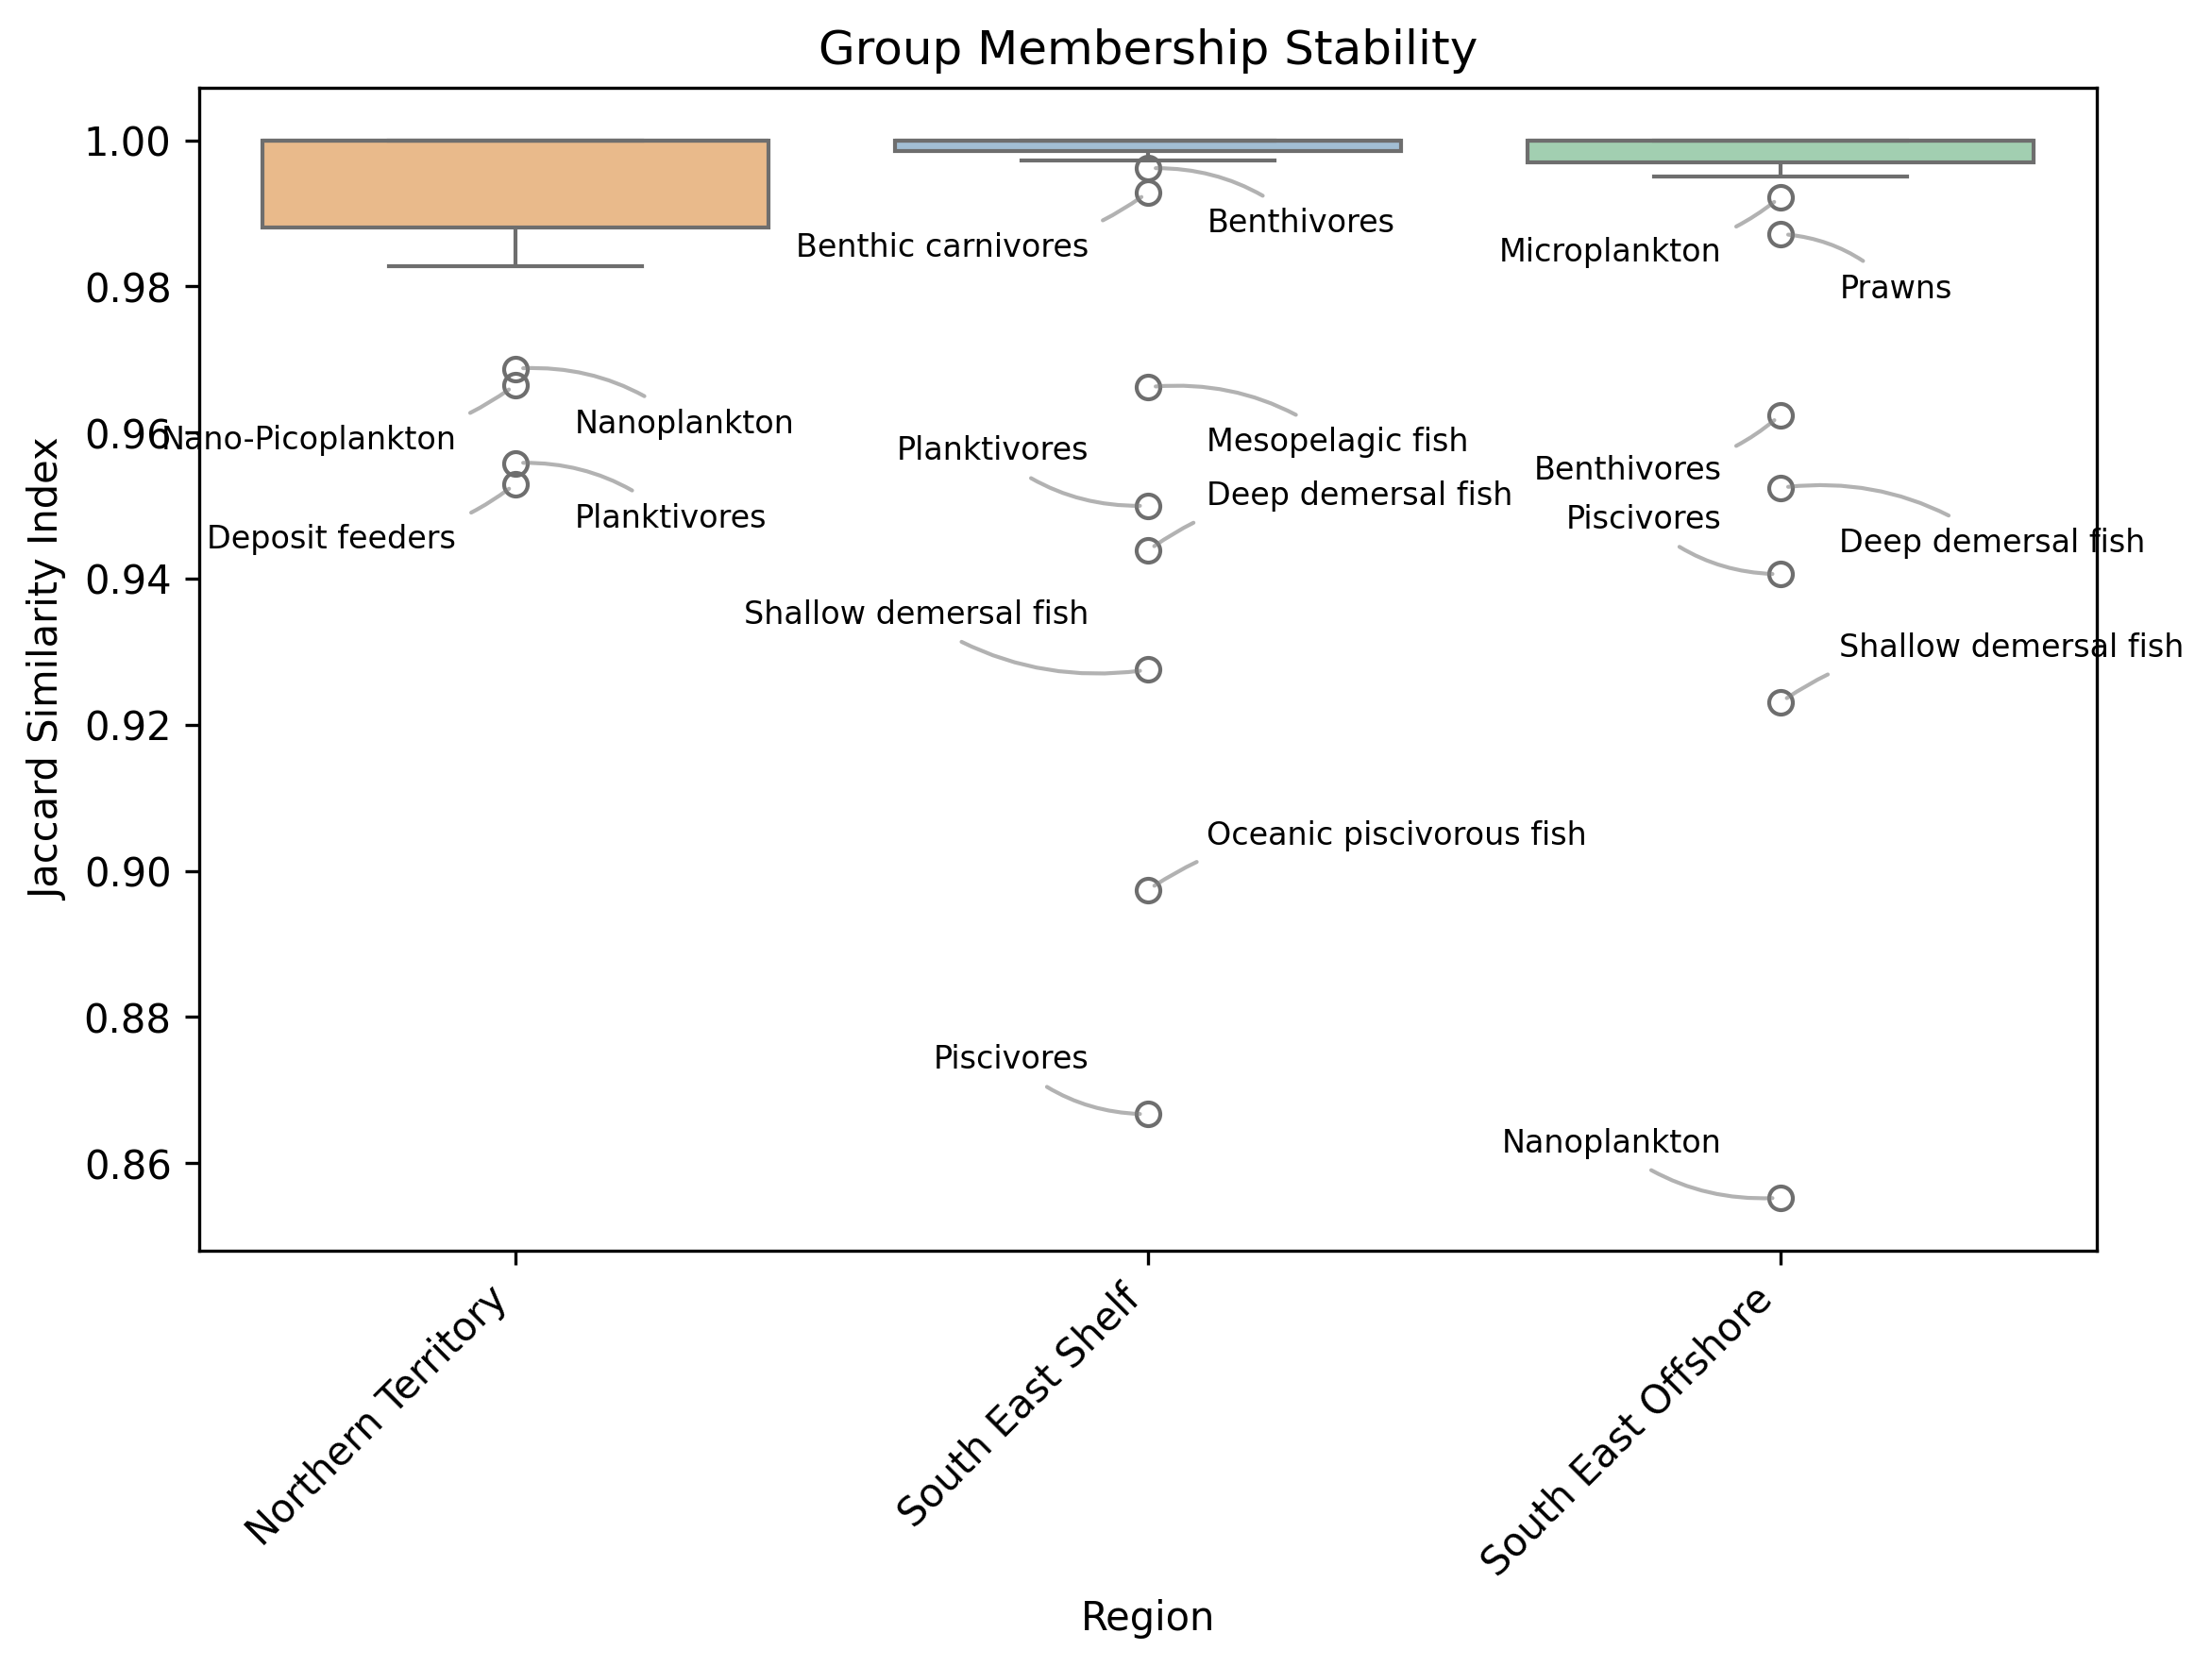
\includegraphics[width=\textwidth]{figures/regional_group_analysis.png}
    \caption{Multi-panel analysis of framework performance across regions. (A) Box plots of functional group sizes (0-3000 species), showing similar median sizes but varying distributions across regions, with outliers indicating some very large groups. (B) Violin plots of species classification consistency (0.4-1.0), where wider sections indicate more species with that consistency score; most species show high consistency (>0.9) with slightly more variation in the Northern Territory. (C) Box plots of group stability measured by Jaccard similarity (0.975-1.000), showing highest stability in South East Offshore and more variable stability in Northern Territory. (D) Box plots of group size variation (standard deviation 0-35), demonstrating larger fluctuations in group membership in the Northern Territory compared to South East regions.}
    \label{fig:regional_analysis}
\end{figure}

\begin{figure}[htbp]
    \centering
    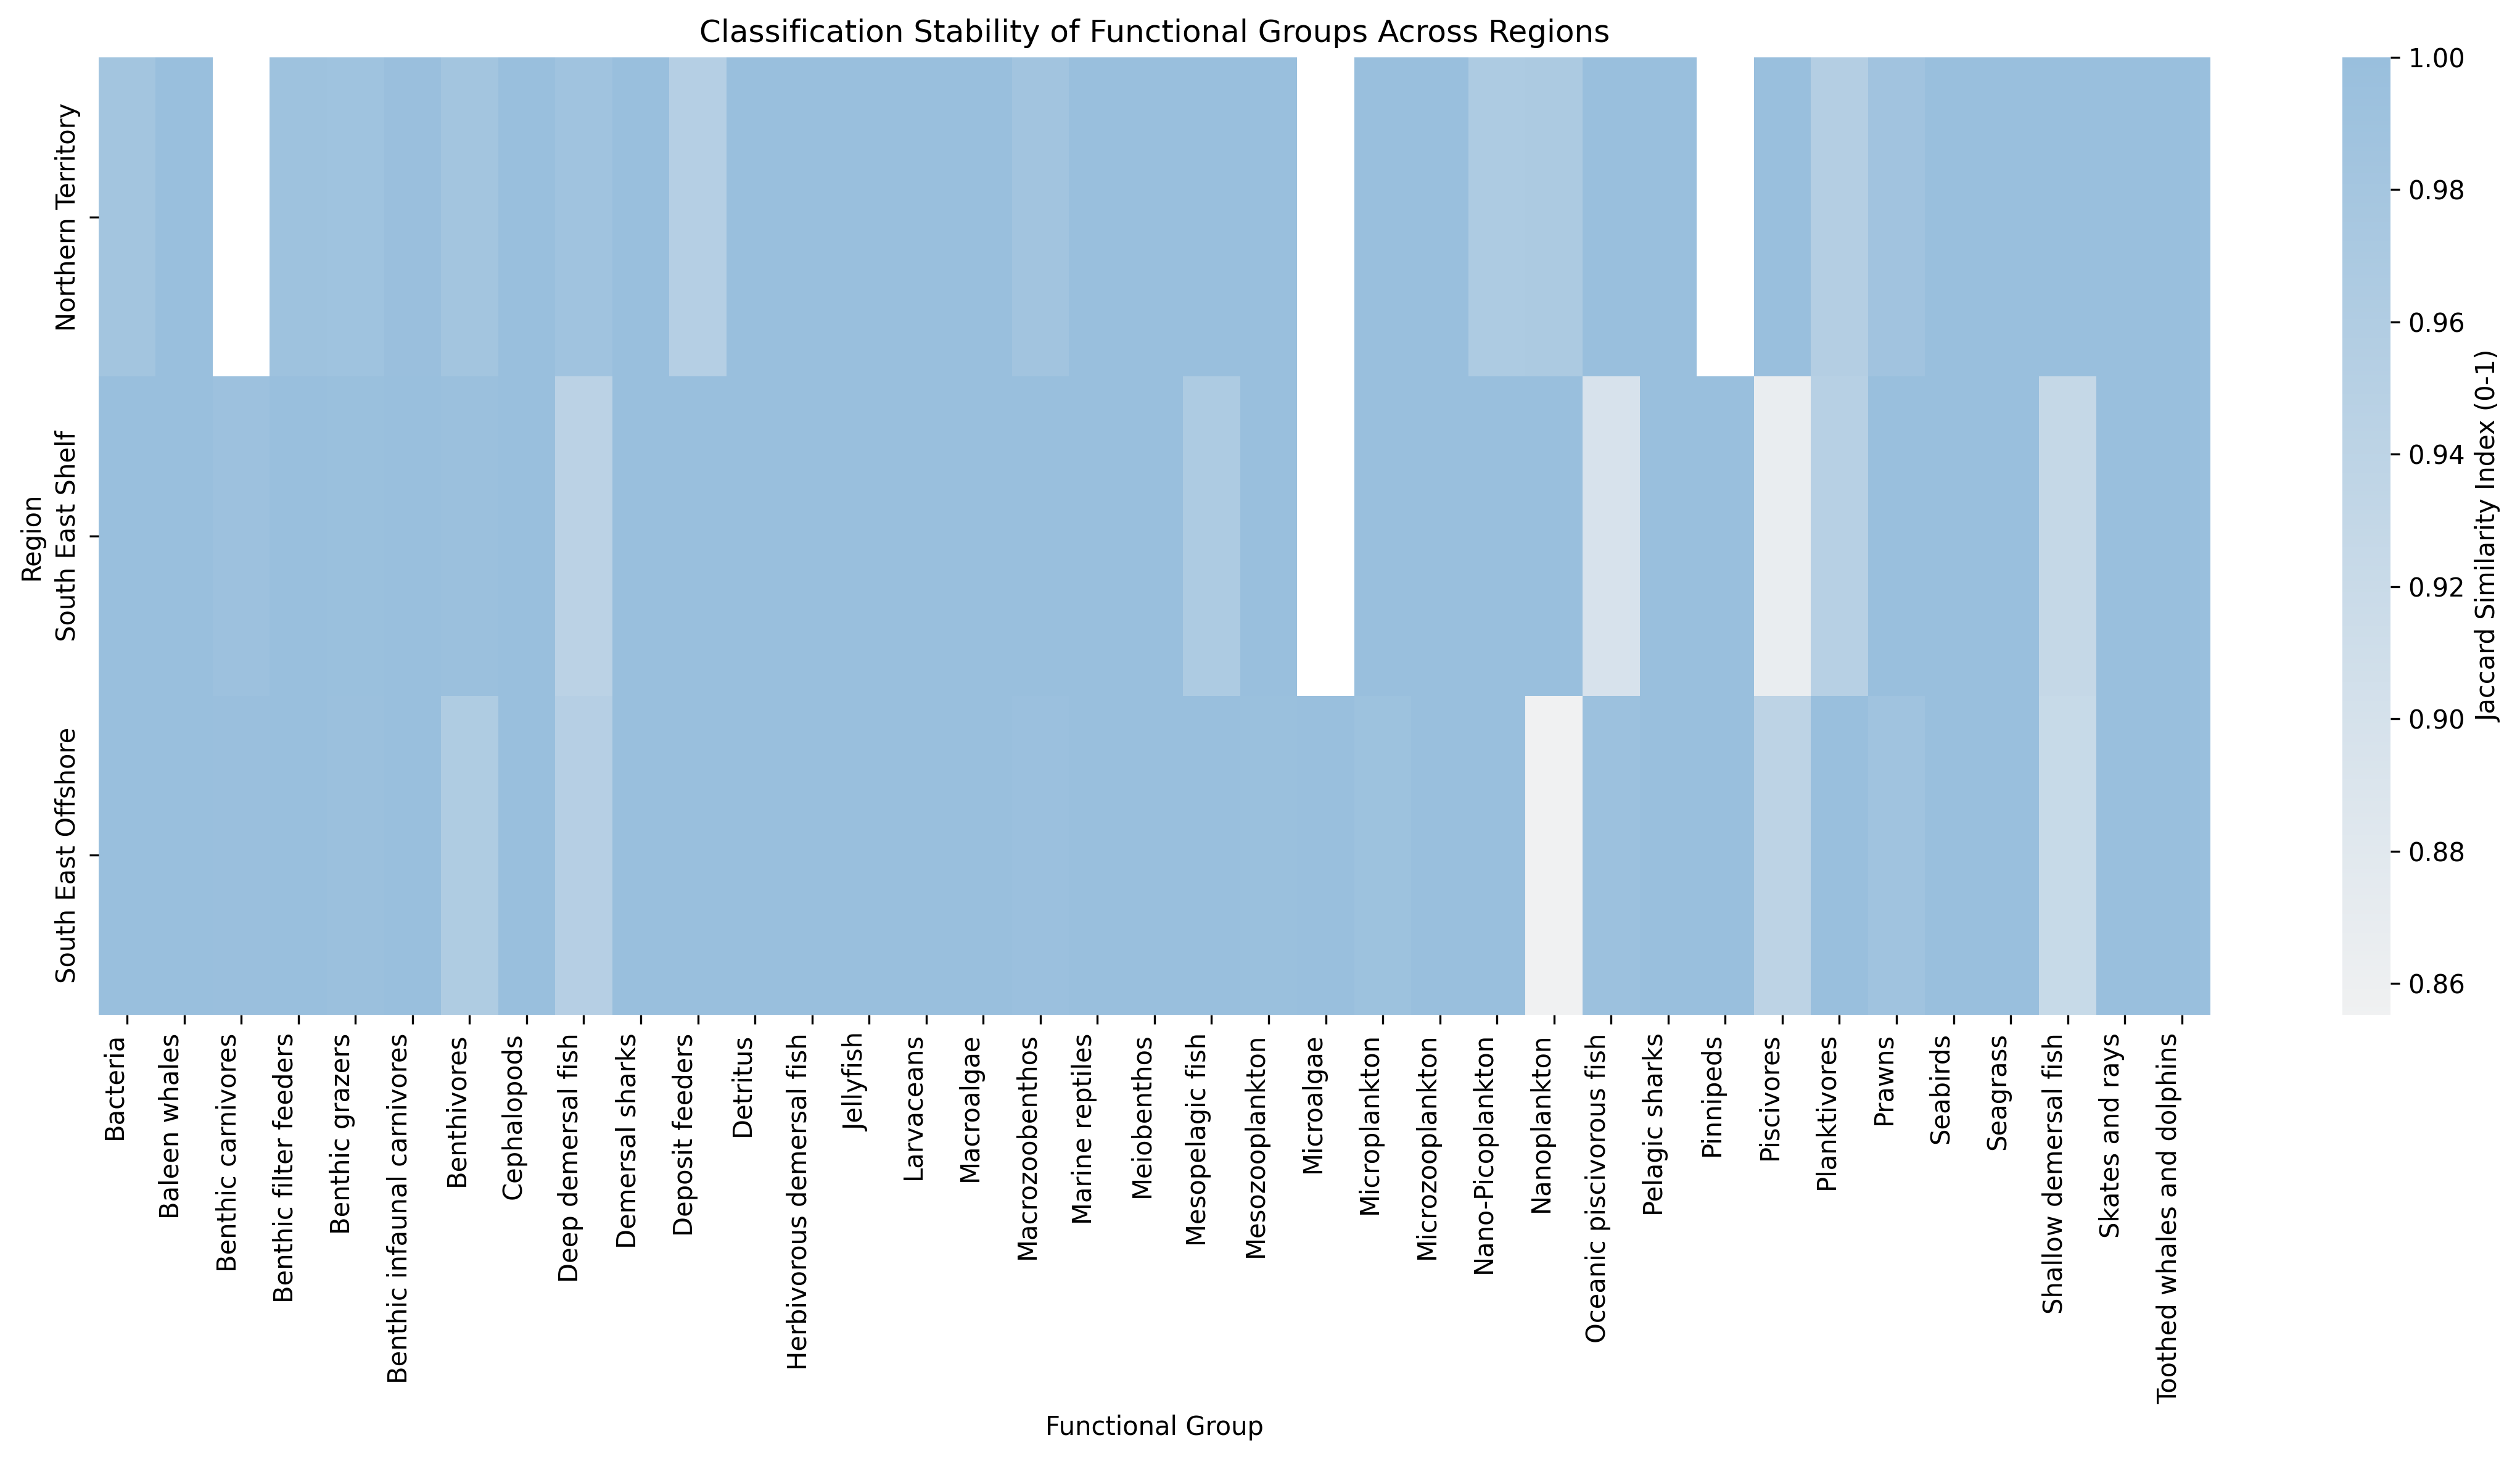
\includegraphics[width=\textwidth]{figures/group_stability_heatmap.png}
    \caption{Heatmap showing the stability of functional group classifications across regions. Each cell displays the Jaccard similarity score (ranging from 0.975 to 1.000) between consecutive framework iterations, where 1.000 indicates perfect consistency in species assignments. Darker red colors represent higher stability (scores near 1.000), while lighter colors indicate more variable classifications (scores closer to 0.975). Most functional groups show high stability (>0.99) across all regions, with occasional variations in groups like benthic grazers and deposit feeders, particularly in the Northern Territory region.}
    \label{fig:stability_heatmap}
\end{figure}

\begin{table}[htbp]
\centering
\caption{Dominant patterns of species classification instability across three study regions. The table presents the most frequent oscillation patterns between functional groups for species that were inconsistently classified across the five framework iterations. For each region, the total number of variably classified species is shown (representing less than 1.1\% of all species), along with the percentage distribution of different oscillation patterns.}
\label{tab:unstable_species}
\small
\begin{tabular}{llcc}
\hline
Region & Most Common Pattern & Count & \% of Total \\
\hline
Northern & Macrozoobenthos $\leftrightarrow$ Benthic infaunal carnivores & 28 & 27.2\% \\
Territory & Benthic filter feeders $\leftrightarrow$ Deposit feeders & 25 & 24.3\% \\
(103 species) & Prawns $\leftrightarrow$ Macrozoobenthos & 21 & 20.4\% \\
& Other patterns & 29 & 28.1\% \\
\hline
South East & Piscivores $\leftrightarrow$ Deep demersal fish & 42 & 33.6\% \\
Inshore & Benthic grazers $\leftrightarrow$ Benthic carnivores & 31 & 24.8\% \\
(125 species) & Planktivores $\leftrightarrow$ Mesopelagic fish & 28 & 22.4\% \\
& Other patterns & 24 & 19.2\% \\
\hline
South East & Benthic filter feeders $\leftrightarrow$ Benthic carnivores & 25 & 28.7\% \\
Offshore & Macrozoobenthos $\leftrightarrow$ Deep demersal fish & 22 & 25.3\% \\
(87 species) & Mesozooplankton $\leftrightarrow$ Macrozoobenthos & 18 & 20.7\% \\
& Other patterns & 22 & 25.3\% \\
\hline
\multicolumn{4}{p{0.95\textwidth}}{\small \textit{Note:} Arrows indicate group assignment oscillation between iterations. Complete species-level data available in Section S3 of the supplementary material.} \\
\hline
\end{tabular}
\end{table}


\subsubsection{Diet Matrix Validation}
The framework demonstrated consistent patterns in diet matrix construction across iterations. Using our stability score metric (where 0 indicates perfect stability and 1 indicates maximum variation), we found that most predator-prey interactions remained highly stable (Figure~\ref{fig:stability_distribution}). The Northern Territory analysis identified 127 predator-prey interactions with a median stability score of 0.18, with 84\% of interactions showing scores below our 0.3 threshold. The South East Inshore region produced 133 interactions with a median stability score of 0.16 (86\% below threshold), while the South East Offshore achieved the highest stability with 147 interactions and a median score of 0.15 (89\% below threshold).

\begin{figure}[htbp]
    \centering
    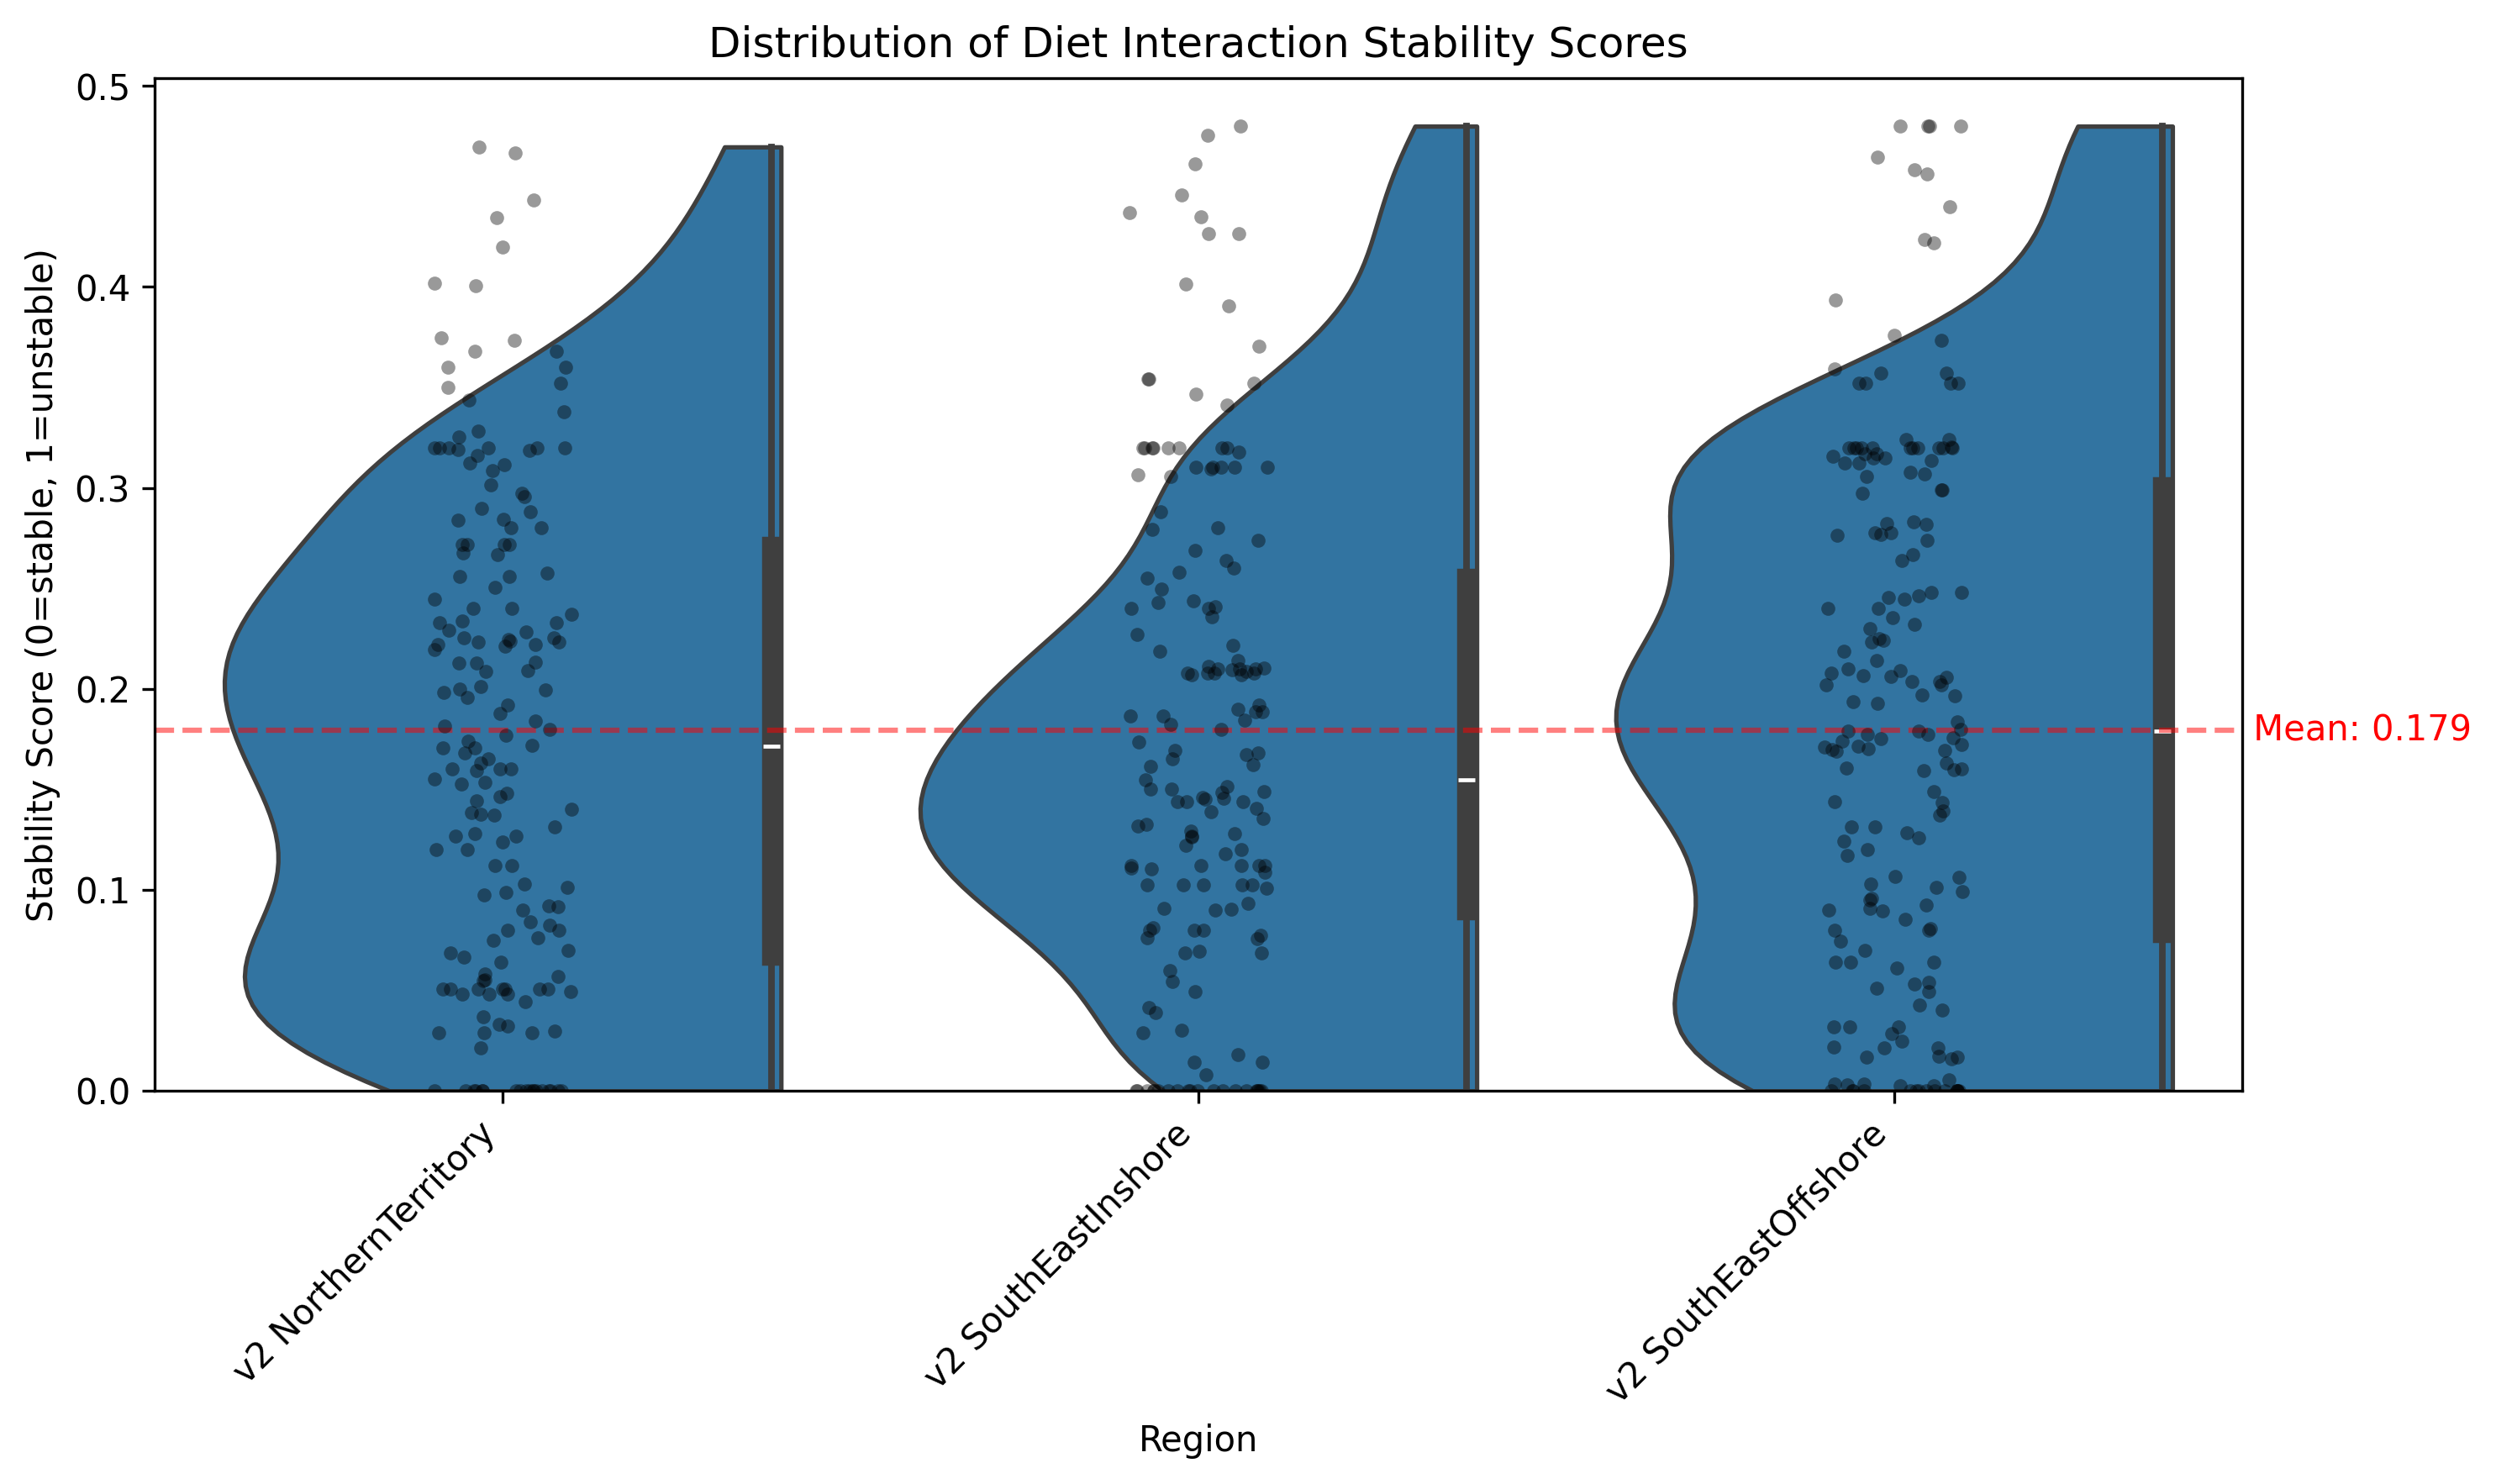
\includegraphics[width=\textwidth]{figures/stability_score_distribution.png}
    \caption{Distribution of diet interaction stability scores across regions. Half-violin plots show the density of stability scores (0=stable, 1=unstable), with embedded box plots indicating quartiles and median. Individual points represent specific predator-prey interactions, and the red dashed line shows the mean stability score across all regions. The distributions are bounded at zero, reflecting perfect stability, with most interactions showing scores below 0.3.}
    \label{fig:stability_distribution}
\end{figure}

Analysis of stability scores by predator group revealed systematic patterns in diet consistency (Figure~\ref{fig:predator_stability}). Lower trophic level groups like nanoplankton and microplankton showed high stability (scores < 0.1) across all regions, reflecting their specialized diets. Mid-trophic level predators such as mesopelagic fish and cephalopods exhibited moderate variability (scores 0.1-0.2), while higher trophic level predators including demersal sharks and benthic carnivores showed the most variation in diet composition (scores > 0.2). This pattern suggests that diet variability increases with trophic level, possibly reflecting the more generalist feeding strategies of higher-level predators. Detailed diet matrices for each region are provided in the supplementary material (Figure~S1).

\begin{figure}[htbp]
    \centering
    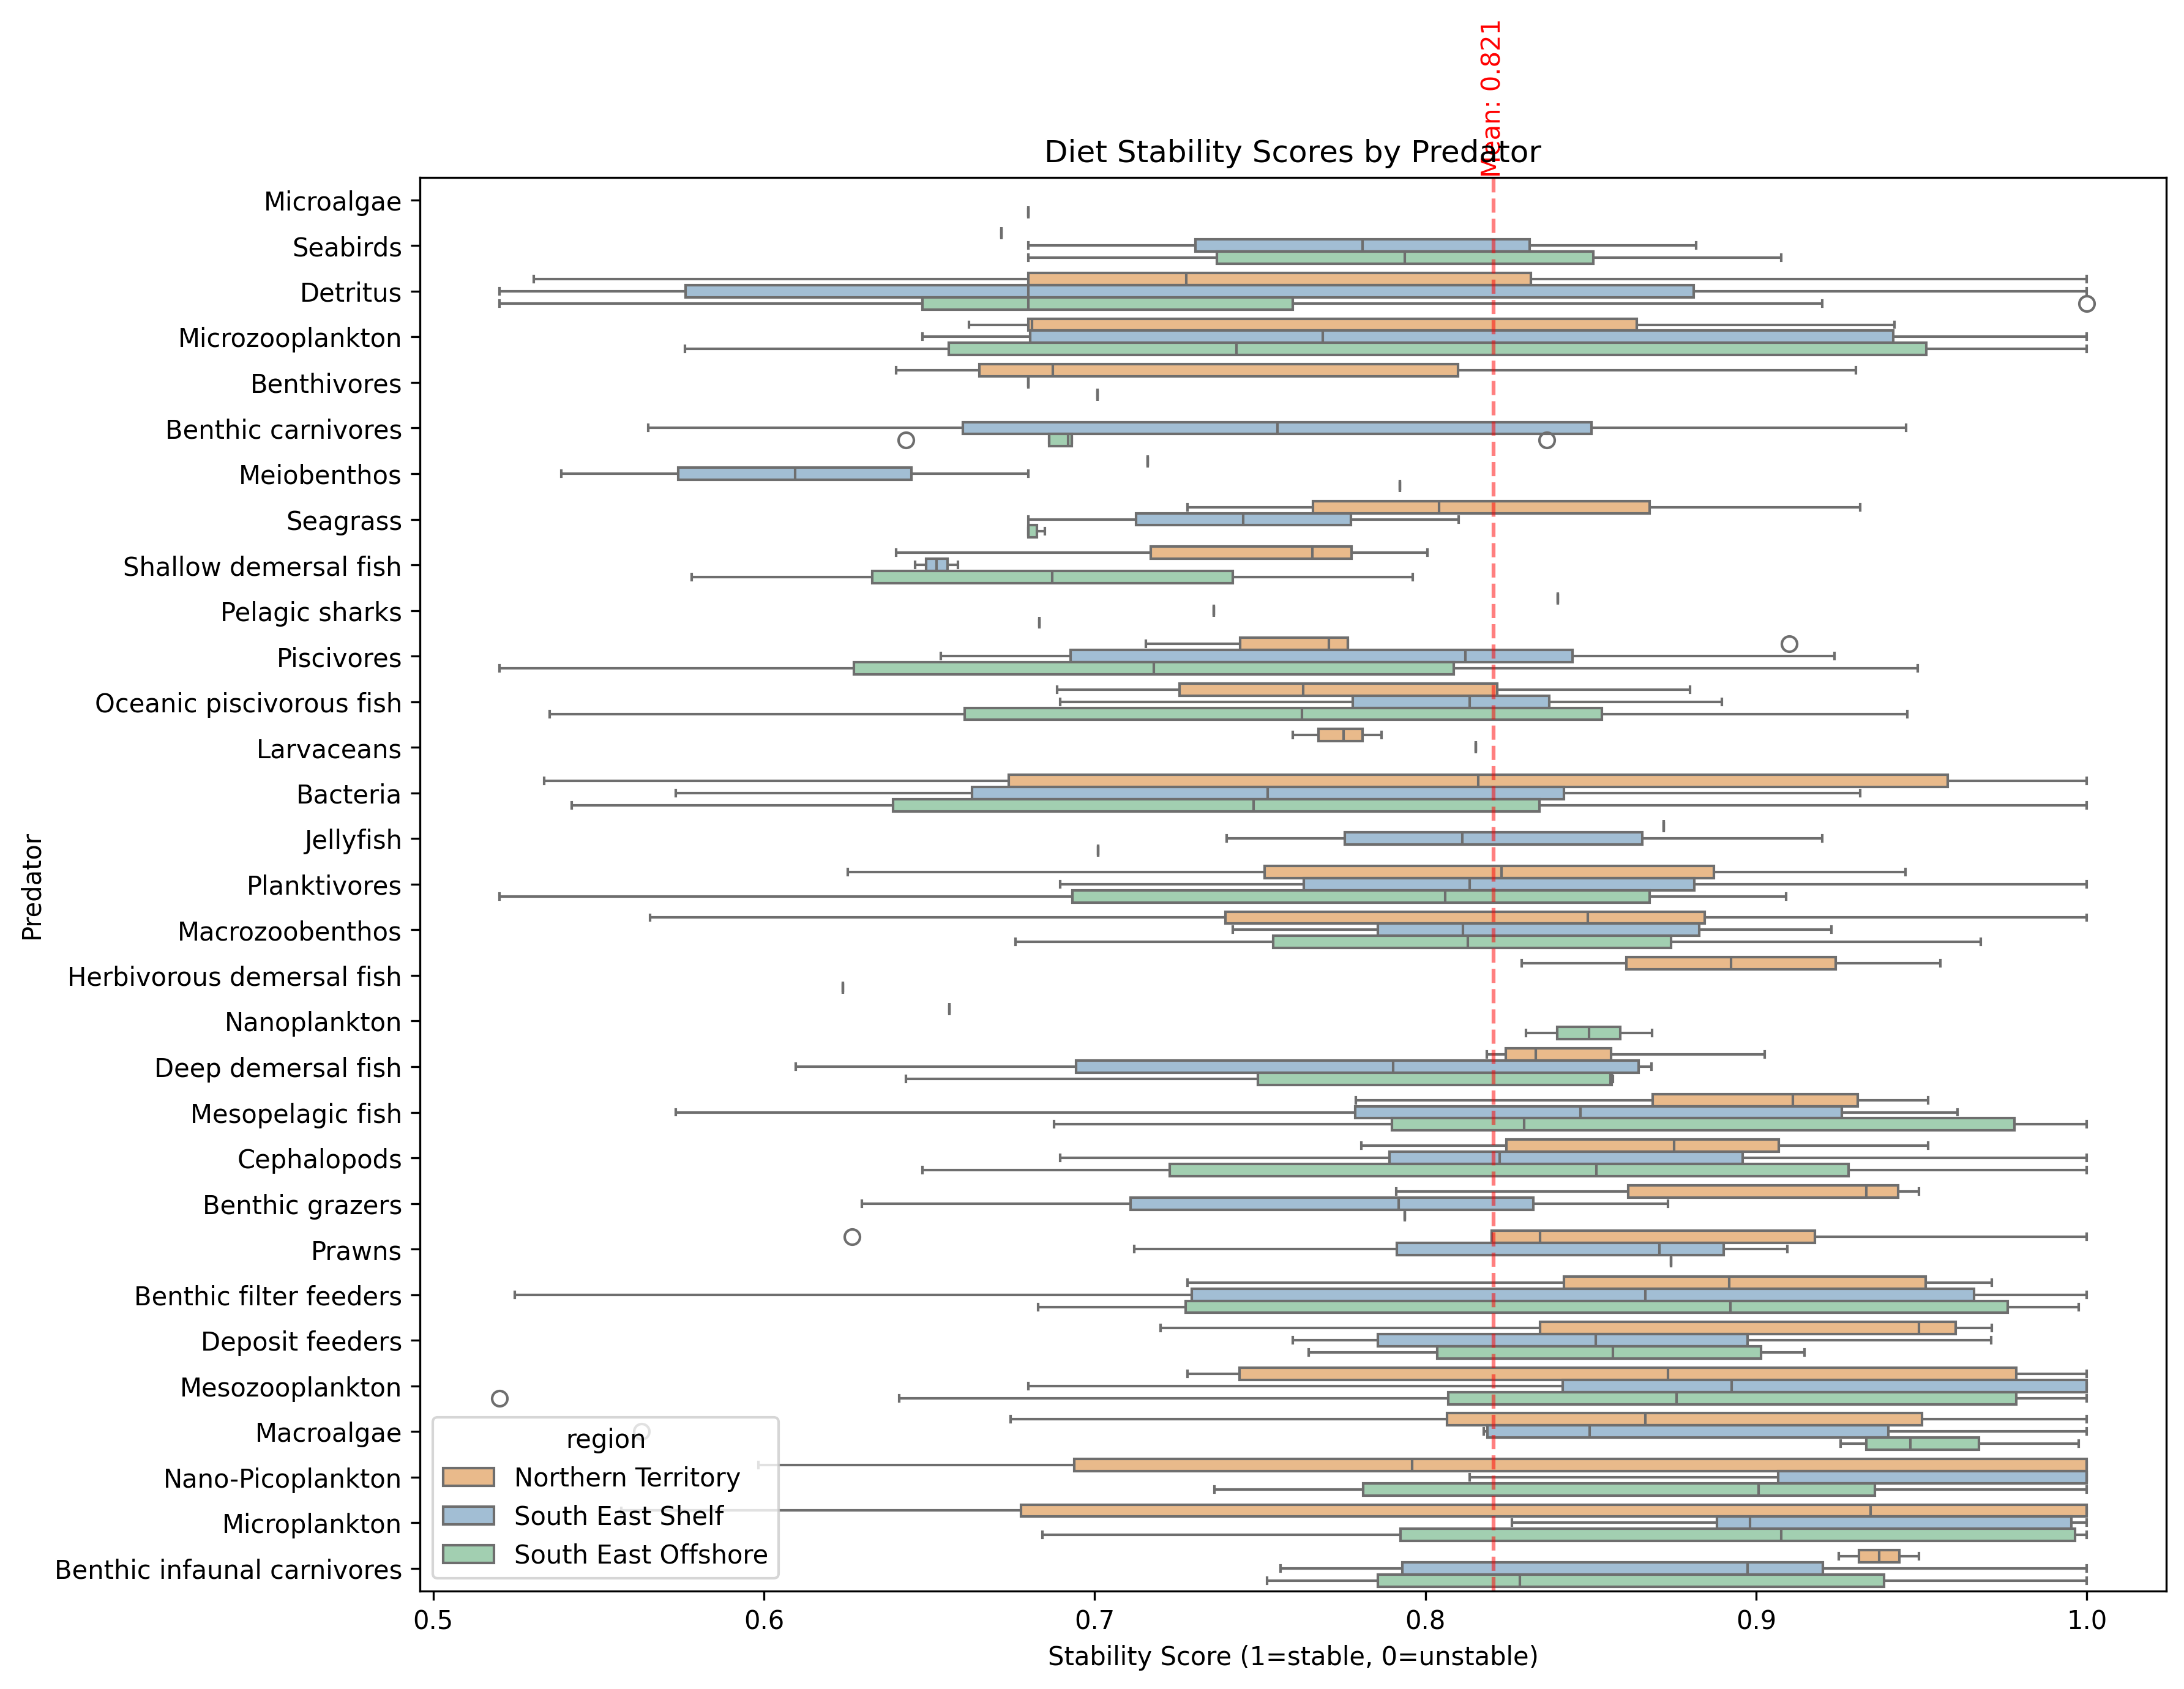
\includegraphics[width=\textwidth]{figures/predator_stability_boxplots.png}
    \caption{Diet stability scores grouped by predator, ordered by median stability. Box plots show the distribution of stability scores for each predator's diet across regions (colored by region). The red dashed line indicates the mean stability score across all predator-prey interactions. Lower scores indicate more consistent diet compositions across framework iterations.}
    \label{fig:predator_stability}
\end{figure}

\subsection{Ecological Findings}

\subsubsection{Trophic Level Patterns}
Analysis of trophic structure revealed significant differences in both the Northern Territory and South East Inshore regions (Kruskal-Wallis H-test, H = 164.0 and 172.0 respectively, p < 0.001 for both). Higher trophic level species, particularly apex predators and specialized feeders, maintained consistent classifications across all regions. In contrast, lower trophic levels showed greater variability, particularly among planktonic and benthic invertebrate groups. Benthivores exhibited the highest variation, ranging from 715 to 788 species between runs, while shallow demersal fish showed moderate variation between 586 and 659 species.

\section{Discussion}

\subsection{AI Framework Consistency}
Our framework demonstrates robust performance in automating the construction of complex ecosystem models across diverse marine environments. The successful processing of over 41,000 species across three distinct regions validates the framework's scalability and broad applicability. The framework's ability to maintain consistent species classifications while adapting to regional ecological differences suggests it effectively captures fundamental ecological relationships.

The computational efficiency analysis reveals important insights about framework scalability. Data harvesting and diet collection emerge as the primary computational bottlenecks, particularly evident in the South East Inshore region's extended processing times. These bottlenecks likely stem from API rate limitations and the complexity of extracting ecological information from diverse data sources. The relatively constant processing times for species identification, grouping, and parameter estimation across regions indicate these components scale efficiently with increasing species counts.

The framework's classification consistency merits particular attention. The high stability scores (98.8-99.6\%) across regions demonstrate reliable species-to-group assignments. The systematic nature of classification inconsistencies provides valuable ecological insights. Species with ambiguous classifications often represent organisms that naturally span multiple ecological niches. For instance, the alternating classifications of anemones between benthic infaunal carnivores and filter feeders reflect their complex feeding strategies. Similarly, the variable classification of flatfishes between benthivore and demersal categories aligns with their known ecological plasticity. These classification patterns suggest the framework captures meaningful ecological uncertainty rather than arbitrary assignment errors.

The diet matrix validation reveals a nuanced picture of trophic relationship stability. The moderate negative correlations between iterations initially appear concerning. However, the high stability of significant feeding interactions (89.8-92.5\%) suggests the framework maintains consistent broad-scale trophic structure while allowing flexibility in fine-scale interactions. This pattern aligns with ecological theory, where core trophic relationships remain stable while peripheral feeding interactions may vary with resource availability and environmental conditions.

The observed trophic level patterns provide compelling evidence for the framework's ecological validity. The consistent classification of higher trophic level species reflects the relatively constrained niches of specialized predators. Conversely, the greater variability in lower trophic level classifications mirrors the natural complexity and adaptability of these groups. The framework's ability to capture this fundamental ecological pattern suggests it successfully incorporates biological realism into its classification decisions.

The regional differences in group size variation and classification stability offer insights into ecosystem complexity. The Northern Territory's higher variation in group sizes and slightly lower classification stability likely reflect the increased ecological complexity of tropical reef systems. The more stable classifications in the South East regions may indicate more clearly defined ecological niches in temperate marine environments. These regional patterns demonstrate the framework's sensitivity to underlying ecological differences while maintaining consistent overall performance.

The reduction from 63 potential functional groups to 34-36 region-specific groups indicates the framework's ability to identify ecologically relevant groupings while avoiding artificial complexity. The statistical consistency across regions suggests these groupings represent fundamental ecological units rather than arbitrary divisions. This optimization of functional group complexity balances model detail with practical utility, a crucial consideration for ecosystem modeling applications.


\subsection{Limitations and Uncertainties}

Our framework faces several AI-specific limitations identified in recent ecological modeling research. The framework's performance depends on the quality and completeness of available training data. The framework's classification patterns showed regional variations in stability, though further research is needed to determine the relationship between data availability and classification performance. This consideration aligns with findings from \cite{Kuhn2024} regarding machine learning applications in fisheries, where data quality significantly impacts model reliability.

A significant limitation of our approach stems from its reliance on Claude 3.5 Sonnet, a closed-source large language model. The proprietary nature of this model introduces uncertainty regarding the training data used in its development and potential biases that may affect ecological interpretations. While our validation demonstrates consistent performance, the inability to examine the model's training data or internal decision-making processes raises important considerations for scientific reproducibility. Future iterations of the framework may benefit from exploring open-source alternatives or implementing multiple model approaches as demonstrated by \cite{Kommineni2024} in their work with various LLMs for biodiversity research.

The framework's interpretability presents another key challenge. While our validation demonstrates robust performance metrics, the underlying AI decision-making processes, particularly in parameter estimation, require careful scrutiny. This challenge mirrors concerns raised by \cite{Fernandes2024} regarding the "black box" nature of AI systems in aquaculture applications. Our framework partially addresses these concerns through explicit uncertainty quantification and validation metrics, but further work is needed to enhance model transparency.

Technical limitations include computational resource requirements and processing time constraints, particularly evident in data harvesting operations. These limitations align with implementation barriers identified by \cite{Fernandes2024}, including acquisition costs and technical expertise requirements. The framework's sensitivity to data availability varies across ecological roles and regions, affecting both classification stability and diet matrix reliability.

\subsection{Applications for EBFM}

The framework offers significant practical value for ecosystem-based fisheries management through several key capabilities. Managers can now construct initial EwE models for new regions in days rather than months, enabling faster response to management needs. This addresses a key bottleneck identified by \cite{Zheng2023} in marine resource management. The framework's explicit quantification of uncertainty in species classifications and trophic relationships enables managers to identify areas requiring additional data collection or careful monitoring, following approaches recommended by \cite{Kuhn2024}. 

The demonstrated adaptability across diverse ecosystems enables customization for specific regions while maintaining methodological consistency, supporting standardized approaches to ecosystem management across jurisdictions. Through systematic processing of available data, the framework also reveals specific areas where additional research or monitoring would most improve model reliability, aligning with recent work by \cite{Chen2024} on marine protected area management.

\subsection{Future Directions}

Future development should focus on several key areas to enhance the framework's utility and reliability. Integration with emerging marine AI systems, such as specialized models like MarineGPT \citep{Zheng2023} and multimodal frameworks like LITE \citep{Li2024}, could enhance the framework's capabilities in processing region-specific information and handling incomplete data. The LITE framework's success in combining semantic time-series with temporal trend images suggests promising directions for improving our framework's robustness to data gaps and distribution shifts. Their sparse Mixture-of-Experts approach to handling incomplete features could particularly benefit our diet matrix construction process. Implementation of standardized evaluation frameworks, such as those proposed in the ELLE dataset \citep{Guo2025}, would enable more rigorous assessment of the framework's performance across different ecological contexts. Development of improved visualization and explanation tools for AI decision-making processes would address current limitations in model transparency and support broader adoption in management contexts.

\subsection{Conclusion}

Our validation analysis demonstrates both the capabilities and limitations of AI-assisted ecosystem modeling. The framework shows remarkable stability in many aspects while highlighting areas of ecological uncertainty that deserve attention. The clear regional patterns in performance suggest that the approach can adapt to different ecological contexts while maintaining scientific rigor. These findings support the framework's utility for ecosystem-based management while providing clear directions for future improvement.

The observed trade-offs between consistency and complexity reflect fundamental challenges in ecosystem modeling rather than simple methodological limitations. By quantifying these trade-offs and their regional variations, our analysis provides a foundation for more informed application of ecosystem models in fisheries management. As marine ecosystems face increasing pressures from climate change and human activities, this understanding of model behavior and limitations becomes increasingly crucial for effective ecosystem-based management \citep{Geary2020}.


\section*{Acknowledgements}
[Add acknowledgements here]

\section*{Data Availability}
The complete codebase, including all scripts, configuration files, and analysis tools, is available at [GitHub repository URL]. The validation framework, including reference group definitions and classification rules, is documented in the project repository to ensure reproducibility.

\section*{Author Contributions}
SS: Conceptualization, Methodology, Software, Validation, Formal analysis, Investigation, Resources, Data Curation, Writing - Original Draft, Writing - Review \& Editing, Visualization, Project administration. BF: Validation, Writing - Review \& Editing, Supervision, Funding acquisition. FB: Methodology, Software, Validation, Writing - Review \& Editing, Supervision. CB: Investigation, Validation, Writing - Review \& Editing. RB: Investigation, Validation, Writing - Review \& Editing. JPG: Investigation, Validation, Writing - Review \& Editing. JS: Conceptualization, Validation, Investigation, Writing - Review \& Editing. RS: Investigation, Validation, Writing - Review \& Editing. RT: Methodology, Software, Validation, Investigation, Writing - Review \& Editing, Supervision, Funding acquisition.

\section*{Statement on the Use of Generative AI}
Generative AI tools, specifically Claude Sonnet 3.5, were utilized in the preparation of this manuscript to assist with tasks such as language refinement, text structuring, and summarization. All scientific content, data interpretation, and conclusions were independently developed and verified by the authors to ensure accuracy and integrity.

\bibliographystyle{apalike}
\bibliography{references}

\clearpage
\section*{Supplementary Material}

% Create new counter for supplementary sections
\newcounter{suppsection}
\newcounter{suppsubsection}[suppsection]
\newcounter{suppsubsubsection}[suppsubsection]

% Reset counters
\setcounter{suppsection}{0}
\setcounter{figure}{0}
\setcounter{table}{0}

% Define supplementary numbering format
\renewcommand{\thesuppsection}{S\arabic{suppsection}}
\renewcommand{\thesuppsubsection}{S\arabic{suppsection}.\arabic{suppsubsection}}
\renewcommand{\thesuppsubsubsection}{S\arabic{suppsection}.\arabic{suppsubsection}.\arabic{suppsubsubsection}}
\renewcommand{\thefigure}{S\arabic{figure}}
\renewcommand{\thetable}{S\arabic{table}}

% Redefine section commands for supplement
\let\oldsection\section
\let\oldsubsection\subsection
\let\oldsubsubsection\subsubsection

\renewcommand{\section}[2][\empty]{%
  \refstepcounter{suppsection}%
  \ifx\empty#1
    \oldsection*{\thesuppsection\quad#2}%
  \else
    \oldsection*{\thesuppsection\quad#2\label{#1}}%
  \fi
}

\renewcommand{\subsection}[1]{%
  \refstepcounter{suppsubsection}%
  \oldsubsection*{\thesuppsubsection\quad#1}%
}

\renewcommand{\subsubsection}[1]{%
  \refstepcounter{suppsubsubsection}%
  \oldsubsubsection*{\thesuppsubsubsection\quad#1}%
}

% Start new page numbering for supplement
\setcounter{page}{1}
\renewcommand{\thepage}{S\arabic{page}}

\section{Data Harvesting Implementation}\label{supp:data_harvesting}

Our data harvesting system employs DuckDB for efficient querying of PARQUET files, enabling complex joins and aggregations without full memory loading. For species matching across databases, we use structured SQL queries that join on concatenated genus and species names:

\begin{verbatim}
SELECT * FROM sealifebase_df
WHERE SpecCode = {spec_code}
AND PreyStage LIKE '%adult%'
AND PredatorStage LIKE '%adult%'
\end{verbatim}

When combining interaction data from GLOBI with diet information, we implement a comprehensive interaction mapping system that creates bidirectional records:

\begin{verbatim}
interaction_data[source_group]['preys_on'][target_group] = count
interaction_data[target_group]['is_preyed_on_by'][source_group] = count
\end{verbatim}

Our data cleaning protocol standardizes types by converting numerical values to consistent formats and timestamps to ISO format. We handle null values by removing empty values, `NA' strings, and null entries while preserving data structure. Source tracking maintains database origin information for all data points.

The system implements file locking mechanisms for concurrent access, with separate locks for species data and interaction networks. We use exponential backoff retry logic for API interactions, with configurable parameters including maximum retries (5), initial delay (1 second), and maximum delay (60 seconds).

The completion check system verifies the presence of required fields including:
\begin{itemize}
\item Complete taxonomic hierarchy
\item Species-specific database records (when available)
\item Interaction data
\item Source attribution
\item Data quality indicators
\end{itemize}

The final JSON output maintains a consistent structure across all species entries, facilitating automated processing in subsequent framework stages.

\section{Diet Matrix Analysis}\label{supp:diet_matrix}


\begin{landscape}
  \begin{figure}[p]
      \centering
      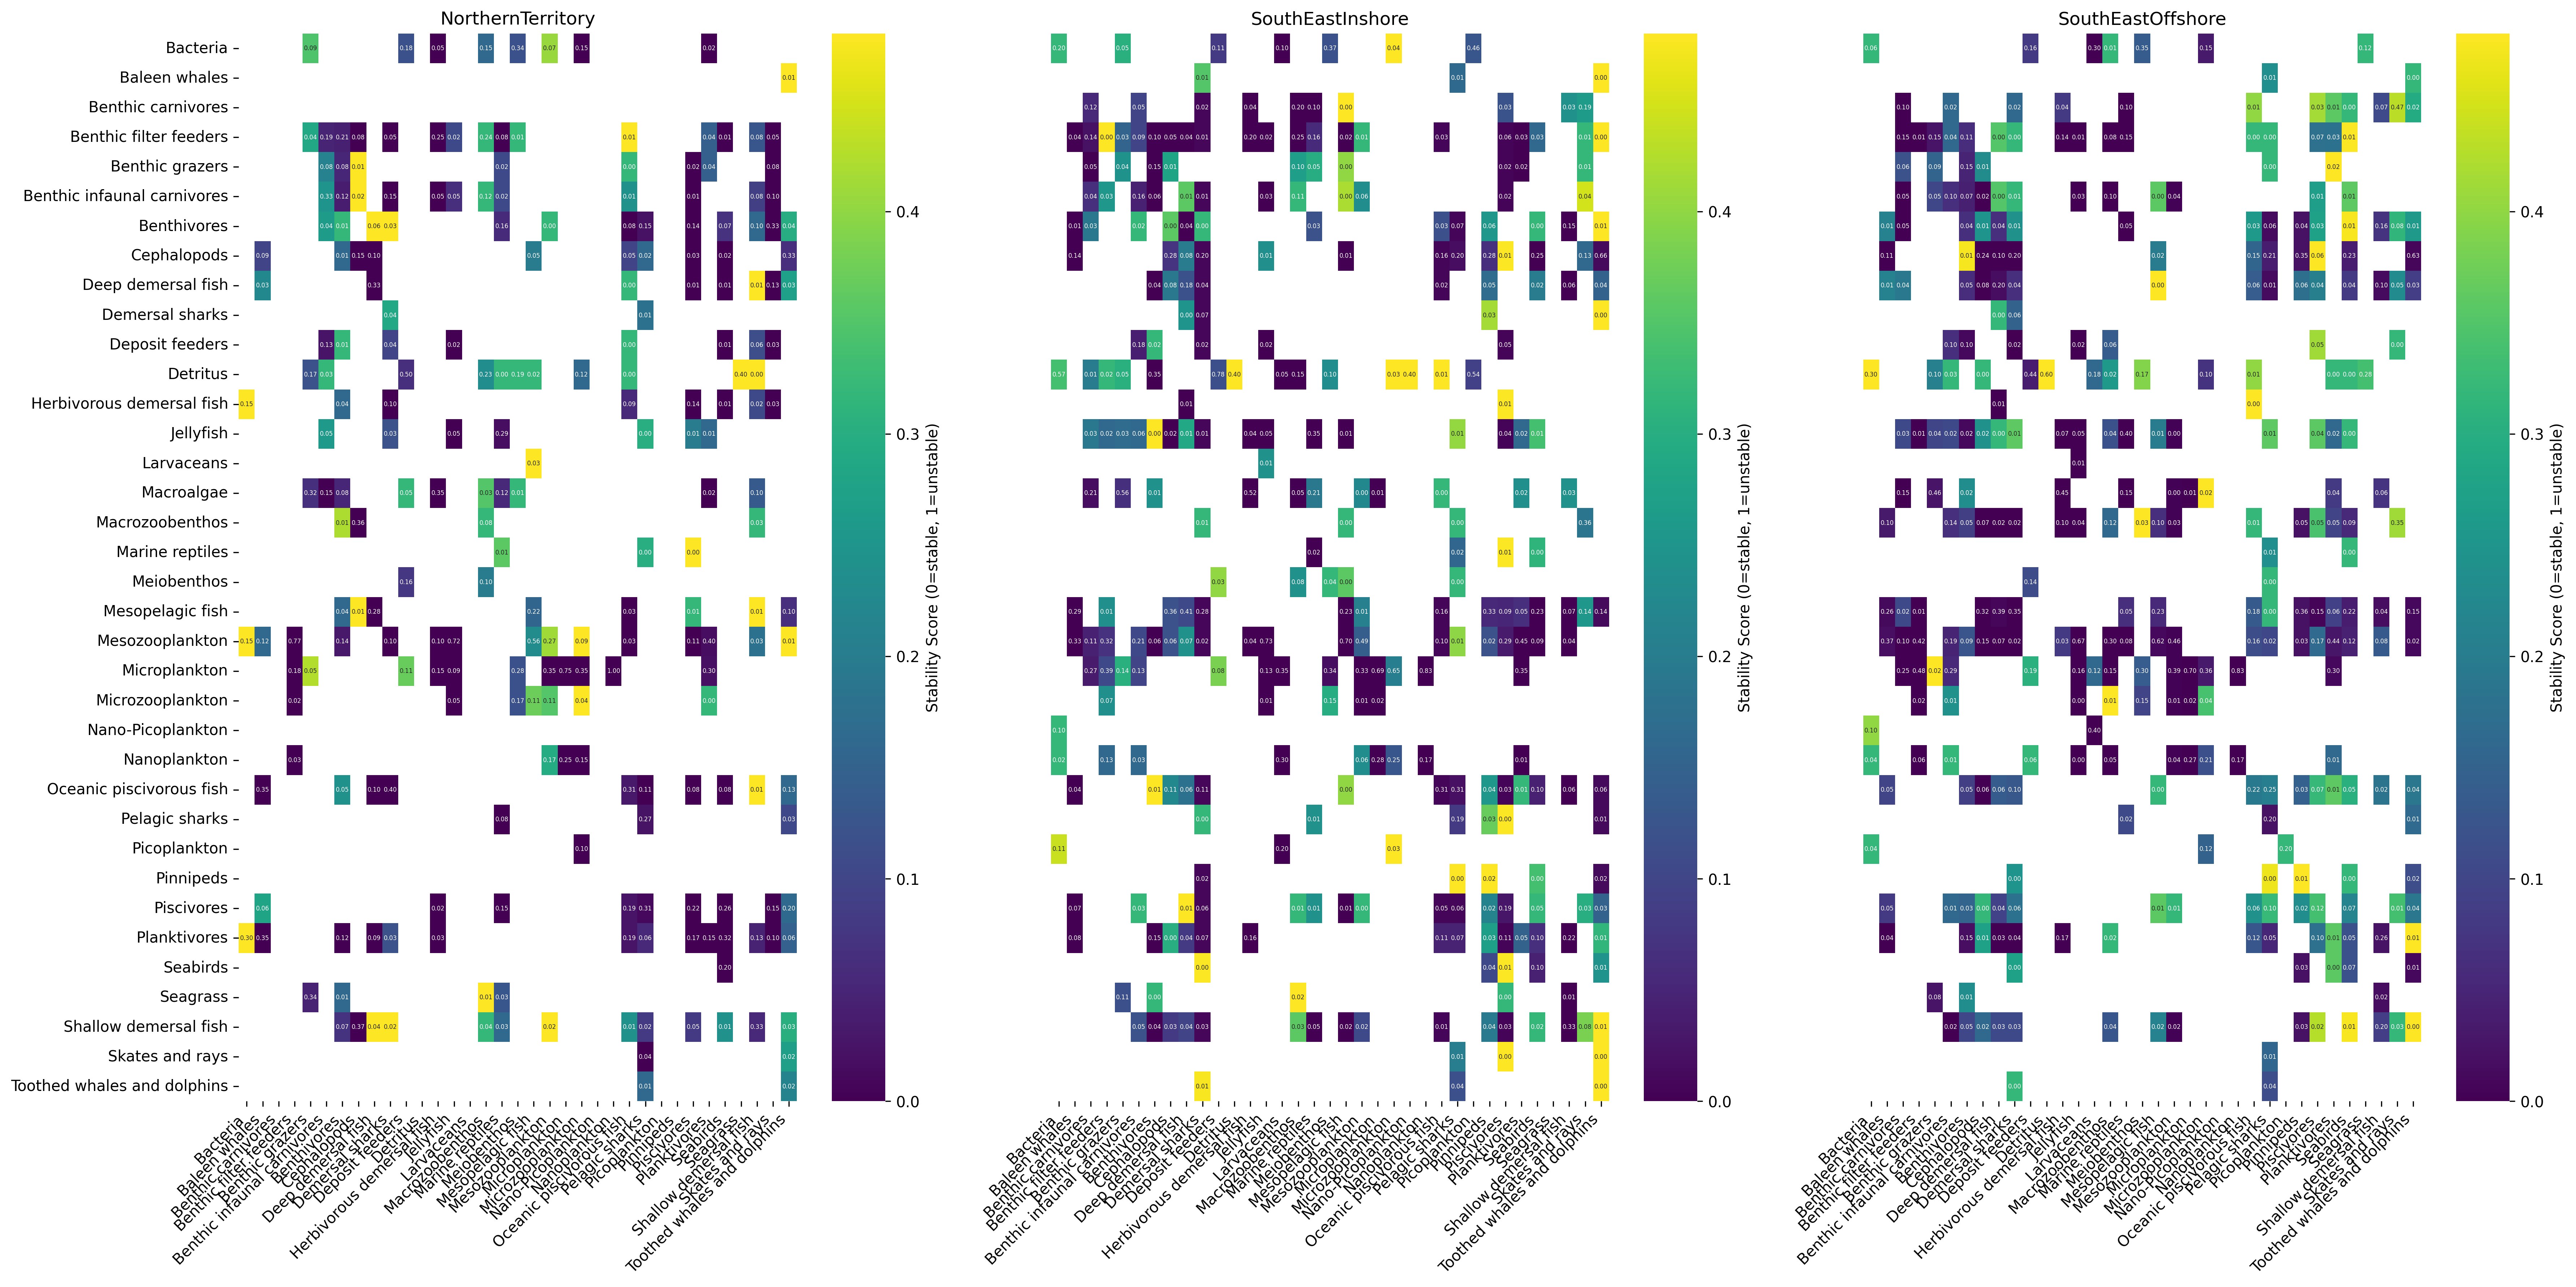
\includegraphics[width=\linewidth]{figures/diet_interaction_heatmap.png}
      \caption{Detailed diet matrix consistency across five iterations for each geographic region. Column names represent predator groups and row names represent their prey groups. Numbers in each cell indicate the mean diet proportions across five iterations, while cell colors indicate the stability score (0-1, where 0 represents perfect stability and 1 represents maximum variation). White cells represent absent feeding relationships. This comprehensive visualization complements the stability score distributions and predator-specific analyses presented in the main text (Figures 4 and 5).}
      \label{fig:diet_matrix_supp}
  \end{figure}
  \end{landscape}
  
  \section{Technical Implementation}\label{supp:technical_implementation}
  \subsection{Default Grouping with Descriptions}
  
  Table \ref{tab:functional_groups} presents the complete template of potential functional groups used by the system. This template serves as a reference for group classification, though the system can create new groups or modify existing ones based on specific ecosystem characteristics.
  
  \begin{longtable}{p{0.3\textwidth}p{0.7\textwidth}}
  \caption{Complete Functional Group Template\label{tab:functional_groups}} \\
  \hline
  \textbf{Group Name} & \textbf{Description} \\
  \hline
  \endfirsthead
  \multicolumn{2}{c}{{\tablename} \thetable{} -- Continued} \\
  \hline
  \textbf{Group Name} & \textbf{Description} \\
  \hline
  \endhead
  \hline
  \multicolumn{2}{r}{{Continued on next page}} \\
  \endfoot
  \hline
  \endlastfoot
  Skates and rays & Bottom-dwelling cartilaginous fish that play a role in controlling benthic prey populations \\
  Nearshore and smaller seabirds & Small gulls, terns etc that feed near shore (possibly include penguins here too) - avian predators that link marine and terrestrial ecosystems \\
  Albatrosses & Large seabirds that forage exclusively at sea, feeding on marine prey (fishes, squids, gelatinous organisms) \\
  Skuas and giant petrels & Large predatory seabirds that feed both at sea and on land, including predation on other birds \\
  Fish-eating pinnipeds & Marine mammals (seals, sea lions) that primarily prey on fish in coastal and pelagic ecosystems \\
  Invertebrate-eating pinnipeds & Marine mammals (particularly Antarctic seals) that primarily feed on krill and other invertebrates \\
  Baleen whales & Large filter-feeding marine mammals that regulate zooplankton populations and contribute to nutrient cycling \\
  Orcas & Apex predators that uniquely prey upon other top predators including marine mammals, sharks, and large fish \\
  Sperm whales & Deep-diving cetaceans that primarily feed on deep-water squid and fish \\
  Small toothed whales and dolphins & Smaller cetaceans that primarily feed on fish and squid in surface and mid-waters \\
  Sea snakes & Marine reptiles that prey primarily on fish, particularly eels and fish eggs \\
  Crocodiles & Large predatory reptiles in coastal and estuarine waters that prey on fish, birds, and mammals \\
  Turtles & Herbivores and omnivores that breed on land \\
  Planktivores & Small fishes that feed on plankton, crucial in transferring energy from plankton to larger predators \\
  Flying fish & Epipelagic fish capable of gliding above the water surface, important prey for many predators \\
  Remoras & Fish that form commensal relationships with larger marine animals, feeding on parasites and food scraps \\
  Large oceanic piscivorous fish & Fish-eating predators in open ocean environments, mid-sized non-migratory species (e.g. barracuda) \\
  Tuna and Billfish & Large oceanic predatory fish, highly mobile, often dive to feed deeper into the water column \\
  Shelf small benthivores & Small bodied fish that feed on benthic organisms, playing a key role in benthic-pelagic coupling, live in shelf waters \\
  Shelf demersal omnivorous fish & Medium sized demersal fish that feed on invertebrates as well as smaller fish, live in shelf waters \\
  Shelf medium demersal piscivores & Medium sized demersal fish living near the bottom in shallow waters, often important in benthic food webs, feed on other fish primarily, live in shelf waters \\
  Shelf large piscivores & Fish-eating predatory fishes found in various marine habitats, important in controlling prey fish populations \\
  Herbivorous demersal fish & Bottom-associated fish that primarily feed on plants, important in controlling algal growth \\
  Slope/deep water benthivores & Small to mid sized fish that feed on benthic organisms and live on the shelf or seamounts \\
  Slope/deep demersal omnivorous fish & Medium sized demersal fish that feed on invertebrates as well as smaller fish, live in slope or seamount waters \\
  Slope/deep medium demersal piscivores & Medium sized demersal fish that feed on other fish primarily, live in slope or seamount waters \\
  Slope/deep large piscivores & Fish-eating predatory fishes found in various marine habitats in deeper water, live in slope or seamount waters \\
  Migratory mesopelagic fish & Fish living in the mesopelagic zone, undertake diel vertical migration, important in energy transfer between depths \\
  Non-migratory mesopelagic fish & Fish living in the mesopelagic zone, non-migratory species, important in energy transfer between depths \\
  Reef sharks & Top predators in coral reef ecosystems, controlling fish populations and maintaining reef health \\
  Pelagic sharks & Open-ocean predators that help regulate populations of fishes and squids \\
  Demersal sharks & Bottom-dwelling sharks, including dogfishes, that control populations of fishes and invertebrates on and near the seafloor \\
  Cephalopods & Intelligent mollusks like squid and octopus, important predators in many marine ecosystems \\
  Hard corals & Reef-building colonial animals that create complex habitat structure through calcium carbonate deposition \\
  Soft corals & Colonial animals that contribute to reef habitat complexity without building calcium carbonate structures \\
  Sea anemones & Predatory anthozoans that can form symbiotic relationships with fish and crustaceans \\
  Hydrothermal vent communities & Specialized organisms living around deep-sea vents, including chemosynthetic bacteria and associated fauna \\
  Cold seep communities & Organisms adapted to methane and sulfide-rich environments on the seafloor \\
  Deep-sea glass sponges & Filter-feeding animals that create complex deep-water habitats and are important in silicon cycling \\
  Sea cucumbers & Deposit-feeding echinoderms important in sediment processing and bioturbation \\
  Sea urchins & Herbivorous echinoderms that can control macroalgal abundance and affect reef structure \\
  Crown-of-thorns starfish & Coral-eating sea stars that can significantly impact reef health during population outbreaks \\
  Benthic filter feeders & Bottom-dwelling organisms that filter water for food, important in nutrient cycling and regulating water quality in various depths - bivalves, crinoids, sponges \\
  Macrozoobenthos & Mobile large bottom-dwelling invertebrates in both shallow and deep waters, important in benthic food webs and bioturbation (predatory or omnivorous) \\
  Benthic grazers & Bottom-dwelling organisms that graze on algae and detritus, influencing benthic community structure \\
  Prawns & Small crustaceans that are important in benthic and pelagic food webs \\
  Meiobenthos & Tiny bottom-dwelling organisms, important in sediment processes and as food for larger animals \\
  Deposit feeders & Animals that feed on organic matter in sediments, important in nutrient cycling \\
  Benthic infaunal carnivores & Predatory animals living within the seafloor sediments \\
  Sedimentary Bacteria & Microscopic organisms crucial in nutrient cycling and the microbial loop in marine ecosystems \\
  Large carnivorous zooplankton & Fish larvae, arrow worms and other large predatory zooplankton \\
  Antarctic krill & Key species in Antarctic food webs, particularly important as prey for whales, seals, and seabirds \\
  Ice-associated algae & Microalgae living within and on the underside of sea ice, important primary producers in polar regions \\
  Ice-associated fauna & Specialized invertebrates living in association with sea ice, important in polar food webs \\
  Mesozooplankton & Medium-sized zooplankton (200 µm to 2 cm) that feed on smaller plankton and serve as food for larger animals \\
  Microzooplankton & Tiny zooplankton (20 µm to 200 µm) that graze on phytoplankton and bacteria, forming a crucial link in the microbial food web \\
  Pelagic tunicates & Including larvaceans, salps, and pyrosomes, important in marine snow formation and carbon cycling \\
  Jellyfish & Predatory gelatinous species \\
  Diatoms & Larger phytoplankton (20 µm to 200 µm), silica dependent important primary producers in marine ecosystems \\
  Dinoflagellates & Mixotrophic species (20 µm to 200 µm) that can switch between primary production and consumption as needed \\
  Nanoplankton & Plankton ranging from 2 µm to 20 µm in size, including small algae and protozoans \\
  Picoplankton & Plankton ranging from 0.2 µm to 2 µm in size, including both photosynthetic and heterotrophic organisms \\
  Microalgae (microphytobenthos) & Microscopic algae that live on the seafloor or attached to other organisms \\
  Pelagic bacteria & Watercolumn dwelling bacteria, consume marine snow amongst other things \\
  Seagrass & Marine flowering plants that form important coastal habitats and nursery areas \\
  Mangroves & Salt-tolerant trees forming critical coastal nursery habitats and protecting shorelines \\
  Salt marsh plants & Coastal vegetation adapted to periodic flooding, important in nutrient cycling and shoreline protection \\
  Macroalgae & Seaweeds of various sizes that provide habitat and food for many species, including both canopy and understory forms \\
  Symbiotic zooxanthellae & Photosynthetic dinoflagellates living within coral and other marine invertebrates \\
  Cleaner fish and shrimp & Species that remove parasites from other marine animals, important in reef health \\
  Discards & Carrion and freshly discarded material from fisheries activities \\
  Detritus & Labile components of natural death and waste \\
  \end{longtable}
  
  \subsection{Retrieval-Augmented Generation Implementation}\label{supp:rag_implementation}
  
  We implement a retrieval-augmented generation system using ChromaDB for vector storage and document management. Document processing begins with LlamaParse conversion of source materials to markdown format, preserving structural elements while enabling consistent text extraction across document types. We segment documents using a token-aware chunking strategy with a 2000-token maximum size, determined through empirical testing to balance context preservation with model limitations.
  
  Document processing follows a two-phase approach. The initial phase generates embeddings for each document chunk using Azure OpenAI's text-embedding-3-small model, storing them in ChromaDB's PersistentClient. The system maintains an indexed\_files.json registry to track processed documents. The second phase handles incremental updates, identifying and processing only new content when documents are added to the source directory.
  
  For diet composition analysis, we implement a two-stage query process. The first stage employs a simple query to retrieve relevant document chunks:
  
  \begin{prompt}
  What do [group] eat?
  \end{prompt}
  
  The system embeds this query using the same Azure OpenAI model and performs vector similarity search to identify relevant document chunks. These results combine with structured data sources including species occurrence frequencies, food category classifications, and GLOBI interaction data to form a comprehensive input for the second stage.
  
  We implement comprehensive error handling throughout the pipeline. The system employs exponential backoff retry logic for API interactions, with configurable parameters including maximum retries (10), initial delay (1 second), and maximum delay (300 seconds). For model interactions, we utilize LlamaIndex's query engine with zero-temperature sampling to ensure deterministic responses. The system supports multiple language model backends including Claude-3 Sonnet (200k token context), GPT-4, and AWS Claude, enabling flexible deployment based on availability and performance requirements.
  
  The system maintains separate storage contexts for different document collections through ChromaDB's collection management. This separation prevents cross-contamination between knowledge bases while enabling efficient parallel processing. We track document citations throughout the retrieval process, maintaining provenance information for all retrieved content. The complete implementation, including embedding generation, chunking algorithms, and query processing functions, is available in the project repository.
  


\end{document}
